\documentclass[12pt]{report}
\usepackage{suthesis}

% -- Imports --
% (general libraries)
\usepackage[utf8]{inputenc}
\usepackage{times,latexsym,amsfonts,amssymb,amsmath,graphicx,url,bbm,rotating}
\usepackage{multirow,hhline,stmaryrd,bussproofs,mathtools,siunitx}
\usepackage{booktabs,xcolor,csquotes,calligra}

% (custom libraries)  %new
\usepackage{afterpage} %new
\usepackage{longtable} %new

% (inline references)
%\usepackage{natbib}
%\usepackage{tabularx}
\usepackage[hidelinks]{hyperref}
\hypersetup{
    colorlinks=true,
    citecolor=magenta,
    linkcolor=.,
    urlcolor=blue
}

\usepackage{epigraph}
\renewcommand{\epigraphsize}{\normalsize}
\setlength{\epigraphwidth}{0.9\textwidth}

% (tikz)
\usepackage{soul}
\definecolor{light-yellow}{RGB}{255, 255, 153}
\sethlcolor{light-yellow}

% (custom)
% (tweaks)
\definecolor{darkred}{rgb}{0.5451, 0.0, 0.0}
\definecolor{darkgreen}{rgb}{0.0, 0.3922, 0.0}

\def\blue#1{\textcolor{blue}{#1}}
\def\darkblue#1{\textcolor{blue}{#1}}
\def\red#1{\textcolor{red}{#1}}
\def\darkred#1{\textcolor{darkred}{#1}}
\def\green#1{\textcolor{green}{#1}}
\def\darkgreen#1{\textcolor{darkgreen}{#1}}
\def\yellow#1{\textcolor{yellow}{#1}}
\definecolor{burntorange}{HTML}{BF5700}
\def\orange#1{\textcolor{burntorange}{#1}}
\def\gray#1{\textcolor{gray}{#1}}
\def\darkgray#1{\textcolor{darkgray}{#1}}

\newcommand\sys[1]{\textsc{#1}}
\newcommand\longcaption[2]{\caption[#1]{#2}}

% (paper compilation hacks)
\usepackage{cite}
\definecolor{darkblue}{rgb}{0.0,0.0,0.4}


% Common hyphenations
\hyphenation{Text-Runner}
\hyphenation{Verb-Ocean}
\hyphenation{Raj-pur-kar}

%\bibliographystyle{plainnat}


% Comments
\usepackage{xspace}
\usepackage{xargs} % commandx
\setlength {\marginparwidth }{2cm}
\usepackage[colorinlistoftodos,prependcaption,textsize=tiny]{todonotes}
\usepackage{marginnote}
\usepackage{color}
\definecolor{darkgreen}{RGB}{0,100,0}

% Inline comments useful for tables and figures.
\newcommandx{\icmtl}[2][1=]{\todo[inline]{DC: #2}\xspace}
\newcommandx{\icmtm}[2][1=]{\todo[inline]{CM: #2}\xspace}

% Comments for other places.
\newcommandx{\cmtl}[2][1=]{\todo[linecolor=blue,backgroundcolor=blue!10,bordercolor=blue,#1]{DC: #2}\xspace}
\newcommandx{\cmtm}[2][1=]{\todo[linecolor=red,backgroundcolor=red!10,bordercolor=red,#1]{CM: #2}\xspace}

\newcommand\cmb[1]{\marginpar{\tiny\raggedright\textcolor{blue}{\textsf{ DC\@: #1}}}}
\newcommand\cmm[1]{\marginpar{\tiny\raggedright\textcolor{red}{\textsf{\bfseries CM\@: #1}}}}

\usepackage{enumerate}

\setcounter{secnumdepth}{3}

\usepackage{footnote}
\makesavenoteenv{tabular}
\makesavenoteenv{table}

\usepackage{xpinyin}

% -- Document --
\begin{document}

% Title
\title{PREDICTING SEA ICE IN THE ARCTIC WITH SUPERVISED LEARNING}
\author{UCL Candidate Code: KNCM2, }
%\principaladviser{Petros Aristidou}
%\firstreader{John Green}
%\secondreader{John BigBooty}
%\thirdreader{Jane Supernumerary} %if needed
%\fourthreader{Severus Snape} %if needed



% Preface
% (notes: "...submitted..." see line 281~286 of function "titlep" in .sty )
\beforepreface
\hypersetup{linkcolor=magenta}
\prefacesection{Abstract}
Predicting future environmental information is one of the most elusive and long-standing challenges in Artificial Intelligence. This report tries to tackle the problem of predicting the Arctic sea ice: how to implement multiple Machine Learning algorithms. On the one hand, we think that Supervised Learning algorithm can predict the Arctic sea ice level. On the other hand, if we want to build an optimal predictor to ensure that our predictions on the Arctic sea ice are useful to the further future research, we would need an efficient and concise strategy to analyse the performance of different Supervised Learning algorithms. Besides, we need more strategies to analyse different factors related to the level of sea ice.

In this project, we firstly focus on Linear Regression, Penalised linear regression, Penalised Polynomial Regression, Random Forest, and Neural Networks: the most common and famous Supervised Learning algorithms by far. Then, according to the testing results, we will choose a better algorithm after testing the performance to be the algorithm that predicts the Arctic sea ice, both in a normal situation and the selected special situations.

This report consists of two parts. In the first part, we aim to understand the advantages of predicting sea ice of the Arctic and previous research on applying all kinds of algorithms on the related topic, especially predicting the Arctic sea ice or the Antarctic ice sheets. Then we present our efforts at implementing effective Supervised Learning algorithms. 

In the second part of this project, we first get our performance results with different Supervised Learning algorithms by K-fold method. This is the so-called now-forecasting. Then, based on the performance results, we predict the Arctic sea ice for the further ten years with Random Forest with different specific scenarios.
\hypersetup{linkcolor=.}
\prefacesection{Acknowledgements}
\afterpreface
\hypersetup{linkcolor=magenta}



% -- Sections --
\chapter{Introduction}                          % Chapter 1
\label{Chapter1:Intro}
% section:
\section{Motivation} %1.1

The motivation for this project includes attention to one of the most serious environmental risks on the planet in the early 21st century, the accelerating global temperature.


According to the paper from Nature, climate change happened in the past 70 years \cite{parmesan2003globally}. It has already had effects on the environment around us. Glaciers are shrinking and ices are breaking up earlier on the lakes and rivers. 

\begin{figure}[!tbh]
\center
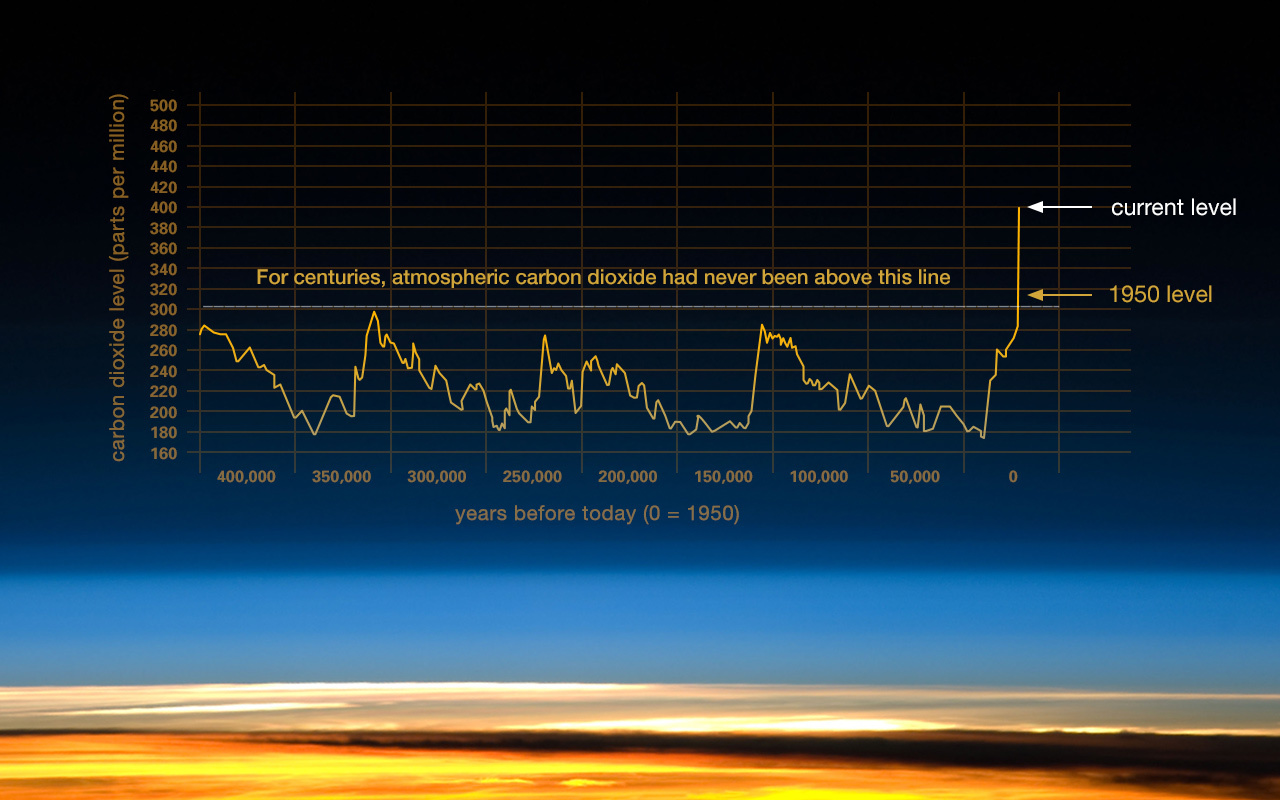
\includegraphics[scale=0.33]{Figure/1.1-NASA-CO2.jpeg}
\longcaption{The evidence that atmospheric CO2 has increased since the Industrial Revolution began}{\label{1.1-NASA-CO2} The evidence that atmospheric CO2 has increased since the Industrial Revolution began. Image courtesy: https://climate.nasa.gov/evidence}
\end{figure}

The greenhouse effect has been working since the formation of the earth. Without the greenhouse effect, the surface of the earth would be extremely cold, the temperature would drop to minus 20°C, the ocean would freeze, and life would not form. Most climate scientists agree that it is the human expansion that causes global warming \cite{epic337530}. As we know, carbon dioxide (CO2) is a significant component of the atmosphere. Atmospheric CO2 concentration has been increased by more than a third since the Industrial Revolution began \cite{epic337530}. More importantly, as shown in Figure \ref{1.1-NASA-CO2}, atmospheric carbon dioxide has exceeded the highest level in the past 400,000 years.

Therefore, what we are facing is not the issue of whether there is a greenhouse effect, but the issue that humans emit a large number of greenhouse gases into the atmosphere through the burning of fossil fuels, causing the drastic greenhouse effect and the earth’s climate.

When the world's average temperature rises by 1°C, huge changes will occur: sea levels will rise, mountain glaciers will retreat, and snow-covered areas will shrink. As the global temperature rises, it will lead to uneven precipitation. In some areas, precipitation increases, while in others, precipitation decreases. For example, the Sahel region in West Africa has been severely arid since 1965, while in North China, precipitation has been decreasing year after year since 1965. Compared with the 1950s, precipitation in North China has been reduced by 1/3, and water resources have been reduced by 1/2. China's annual drought-affected area is about 400 million acres. In normal years, the national irrigation area lacks 30 billion cubic meters of water each year, and the cities lack 6 billion cubic meters of water. 

When the average temperature of the world rises by 3°C, the world will suffer from food shortages. Due to rising temperatures, the global sea level has been rising at a rate of 1 to 2 millimetres per year in the past 100 years. It is expected that the sea level will continue to rise by 30 to 50 centimetres by 2050, which will flood a large amount of low-lying coastal land. In addition, due to climate changes have led to the aggravation of climatic disasters such as droughts, floods, and low temperatures, causing economic losses of more than tens of billions of dollars worldwide each year.


In this report, our team focuses on sea ice in the Arctic. We will look for the elements that we think affect the changes in Arctic sea ice, analyse their influence on the changes in sea ice, and select the two elements that we think are the most important. We will put these two influencing factors into our emergency model, and analyse the impact of significantly changing them on Arctic future sea ice.
\section{Report Outline} %1.2

This thesis consists of two parts --- \sys{Part I Environmental Risks in Supervised Learning: Foundations} and \sys{Part II Scenario: Predicting Arctic Sea Ice in Supervised Learning}.

\sys{Part I} focuses on the task of understanding and building Machine Learning processing flow, including processing to tidy data, so that we are able to predict Arctic sea ice in \sys{Part II}.

\begin{description}
    \item In Chapter~\ref{Chapter2:Review}, we first give an overview of the history and recent development of the field of .... Next we formally define the problem ... and its main categories. We then briefly discuss ....  Finally, we argue ....
    \item In Chapter~\ref{Chapter3:Method}, we present the ..... We begin with describing .... We then introduce ... and we describe .... 
   
\end{description}
\section{Contributions} %1.3
The contributions of this thesis are summarised as follows: 
\begin{itemize}
  \item Our team analysed seven factors influencing the sea ice and gave an result of their correlation relationships.
  
  \item Our team
  
  \item We... 
\end{itemize}

\part{Environmental Risks in Supervised Learning: Foundations}

\chapter{Literature Review}                     % Chapter 2
\label{Chapter2:Review}
% section:
% Chapter 2: Literature Review

\section{Why We Choose to Predict Sea Ice}
The change of Arctic sea ice is a sensitive indicator of climate change. The rate of Arctic sea ice disappearance exceeds even the most pessimistic climate model predictions. The current Arctic summer ice conditions are 30 years earlier than model predictions on average, and seasonal ice-free conditions are happened early \cite{stroeve_frei_mccreight_ghatak_2008}. Therefore, the prediction of sea ice is essential for understanding the future Arctic environment and global changes. Global warming has led to a reduction in sea ice and aggravated the deterioration of the Arctic environment, while the reduction in sea ice, in turn, has accelerated global warming. Increasing concentrations of greenhouse gases are playing an increasingly important role in the disappearance of the Arctic ice cap \cite{kim2019satellite}. Many studies have also linked the loss of sea ice to atmospheric circulation patterns.

\section{How to Predict Sea Ice Level Using Statistical Models}
There are many statistical models that study the relationship between the Arctic sea ice concentration and climate factors. Stroeve et al. pioneered the use of singular value decomposition SVD, empirical orthogonal function EOF and other multivariate analysis techniques, focusing on the relationship between the decline of sea ice concentration in summer and winter and the warming trend and AO driving \cite{stroeve_frei_mccreight_ghatak_2008}. TIvy et al. used the multivariate analysis technique of Code Correlation Analysis (CCA) to compare the SIC value of Hudson Bay in July from 1971 to 2005 by comparing sea surface temperature, position altitude, sea level pressure, and regional surface air temperature. Among them, in the 6-month forecast period, the forecast results are the most accurate. Surface temperature in autumn is the most influential predictor \cite{tivy2011origins}. Ahn et al. introduced the automatic regression integrated moving average (ARIMA) method for the first time into the sea ice concentration statistical model, using seven climatic factors (skin temperature, sea surface temperature, total column liquid water, total column water vapour, and instantaneous moisture flux). It is better at predicting large data sets than the single equation of the ordinary minimum hours (OLS) regression method and has higher accuracy. The average improvement of RMSE is 0.076 \cite{ahn2014statistical}. The forward stepwise regression model is used to predict summer sea ice conditions several months in advance based on four predictors which are winter multi-year combined concentration, total ice concentration in spring, North Atlantic Oscillation Index and East Atlantic Index where $\text{R}{^2}$ value is 90.7\% and $\text{MAE}$ value is 34 \cite{drobot2002practical}. In 2003, it was expanded with multiple linear regression models \cite{drobot2003long}. Finally, in 2007, on this basis, Drobot and others created a multiple linear regression model (MLR) to predict the annual minimum Arctic sea ice range for the monthly interval from February to August. The forecast data is based on the average monthly weighted index of sea ice concentration (WIC), surface skin temperature (WST), surface illuminance (WAL) and surface long-pass volume (WDL). Each MLR model is better than the climatology model \cite{drobot2006long}, but due to insufficient statistical time series modelling, the performance of machine learning models is often better than statistical models.

\section{How to Predict Sea Ice Level Using Machine Learning Models}
Machine learning models are often used to predict Arctic sea ice concentration and Arctic sea ice classification. Chi et al. used a large Arctic sea ice dataset to train a neural network to predict the Arctic sea ice concentration \cite{chi2017prediction}. The neural network prediction results that use long and short-term memory (LSTM) are better than traditional autoregressive (AR) models, and can successfully adapt to long-term data sets. The average monthly forecast error is less than 9\%, but the predictability in summer is low \cite{chi2017prediction}. Choi et al. used artificial neural networks (ANN) to make short-term predictions of the Arctic Sea Ice Concentration (SIC) \cite{choi2019artificial}. Using global SIC data for training will result in higher prediction accuracy than using only Arctic SIC data for training \cite{choi2019artificial}. Shu et al. proposed an object-based random forest (ORF) to classify the ice map types of the Arctic, and the overall classification accuracy was 90.1\%. When providing surface-related values of sea ice density and snow cover, the estimation of ice thickness can be improved \cite{shu2020discrimination}.


\section{How to Predict Sea Ice Level Using Non-Statistical Methods or Non-Machine Learning Methods}
The field of sea ice prediction is very extensive. Since 1979, the satellite-based multi-channel passive microwave imaging system has continuously monitored the Arctic sea ice concentration. Common monitoring systems are Scanning Multichannel Microwave Radiometer (SMMR), Special Sensor Microwave/Imager (SSM/I) and Advanced Microblog Scanning Radiometer (AMSR) \cite{fennig2020fundamental}. Numerical models predict interactions based on physical equations. In the short term, The prediction is usually better than the statistical model. However, it is difficult and expensive to obtain data by physical models \cite{chi2017prediction}. Sea ice retrieval algorithms usually process satellite data, and various sea ice parameters have been determined, such as age, concentration, range, thickness, etc. \cite{chi2017prediction}, but statistical models are usually better than dynamic models \cite{tivy2011origins}.


\chapter{Methodology}                           % Chapter 3
\label{Chapter3:Method}
% section:
\section{Correlation Matrix} %3.1

The correlation matrix is a symmetric matrix. It is a table, which shows correlation coefficients between different variables. It could be used to summarise data, as an input into a more advanced analysis, and as a diagnostic for advanced analyses. The cells in the table indicate the correlation between two variables.

The Pearson's correlation coefficient is the most common correlation coefficient in the correlation matrix. It compares two interval variables or ratio variables. In the correlation matrix, it is also common to use Spearman’s Correlation and Kendall’s Tau-b.

\section{Data} %3.2
For Y-axis, data for Arctic sea ice could be found in National Snow \& Ice Data Centre (NSIDC). For X-axis, data for global CO2 content and Arctic ozone hole area are made available to public via the National Aeronautics and Space Administration (NASA) website. Data for global population were accessed through the Our World in Data website. In addition, data for the different temperatures and rainfall and average daylight of Arctic are provided by National Oceanic and Atmospheric Administration (NOAA) and Weather Atlas website respectively. Furthermore, the data for the global GDP could be found in the world bank website.

All X-axis data are selected from January 1980 to October 2020 and been divided by month. When collecting the data, some data is divided according to the year as a unit, so it is necessary to convert these data into a month as the unit to divide. For example, for the data of population, first subtract the total population in 1980 from the total population in 1979, and then divide the difference into 12 equal parts, and evenly distribute them to each month in 1980, so as to get the 12 months’ data of population in 1980. However, some data sets may lack partial months of data. Thus, first look for data at the same month of other years, and then use the method of means of regression to calculate the missing data.

In order to meet the standard of normalisation, the first data of the set should be 0, which means each data should be subtracted from the value of the first data. Furthermore, all data should be divided by the value of the last data, thus all data would be controlled between 0 and 1, which is convenient for adjusting parameters in subsequent analysis.


%\begin{figure}[!t] % t means top
%    \center
%    \includegraphics[scale=0.5]{img/google_search.pdf}
%    \caption{.....}
%\end{figure}
\section{Feature Description} %3.3

The area of the sea ice in the Arctic is deemed relevant to the following features. The content of carbon dioxide, the area of the ozone hole over the Arctic, the land and ocean temperature in northern hemisphere, the Max/Ave/Min temperature of North Slope Alaska, the rainfall in the Arctic, daylight of Arctic and the population of the world.

\begin{figure}[t]
\center
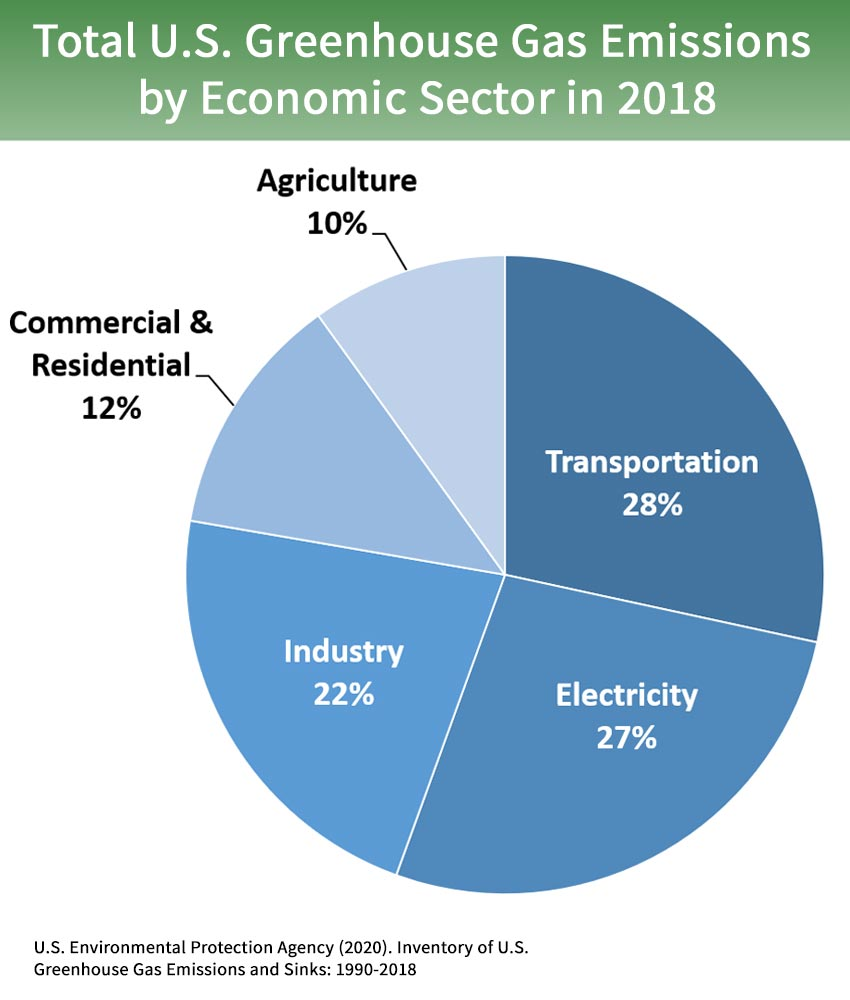
\includegraphics[width = 0.66\textwidth]{Figure/3.3-Overview-USGGE2018.jpg}
\longcaption{Total U.S. Greenhouse Gas Emissions by Economic Sector in 2018}{\label{3.3-Overview-USGGE2018} Total U.S. Greenhouse Gas Emissions by Economic Sector in 2018. Image courtesy: https://www.epa.gov/ghgemissions/sources-greenhouse-gas-emissions}
\end{figure}

Changes in the area of sea ice in the Arctic are believed to be related to the content of carbon dioxide. As shown in Figure \ref{3.3-Overview-USGGE2018}, Carbon dioxide accounts for 81 percentage of greenhouse gases. Thus the main component of greenhouse gases is carbon dioxide, which is also the main cause of the greenhouse effect. According to J.H.Mercer, the greenhouse effect will have a catastrophic impact on the ice sheets \cite{mercer1978west}. Thus the content of carbon dioxide is chosen to be one of the features.

In addition, according to the results of the common correlated effects mean group (CCEMG) estimator, the GDP growth and the population size influence CO2 emission levels positively and significantly, at both the global and regional levels \cite{DONG2018180}. In that case, the GDP growth and the population size would have impact on the ice sheets.

The ozone hole area is also considered to be related to the area of sea ice in the Arctic. In 2010, Sigmond and Fyfe found that the ozone depletion leads to a positive SAM response in austral summer, which induces sea ice melt \cite{sigmond2010has}. In that case, changes in the size of the ozone hole would also affect the changes in sea ice area. Thus the ozone hole area is chosen to be one of the features.

Furthermore, the temperature is deemed to be related to the area of sea ice in the Arctic. According to Ditlevsen and Grinsted's research, by considering a minimal model of an ice sheet, it shows that fluctuating temperatures have an effect on the mass balance and thus on the steady-state volume of the ice sheet \cite{mikkelsen2018influence}. Thus the temperature is considered to be a feature.

Changes in the area of sea ice in the Arctic are also believed to be related to the rainfall. According to Bromwich and Robasky, the increased precipitation may reduce the net loss of ice sheets area or even turn it into net gain \cite{Bromwich1993RecentPT}.Thus rainfall is considered to be a feature.

The amount of daylight in the Arctic is also believed to be related to the area of ice sheets. The Arctic has polar day and polar night phenomena, so there is periodicity in the phenomenon of daylight. As shown in Figure.....

% 这里添加一个光照周期的图


The periodicity of polar day and night and the thermal effect of light.

\section{Model Accuracy} %3.4

In this research, Mean Squared Error function (MSE) is used to test the model accuracy.

The Mean Squared Error function is generally used to detect the deviation between the predicted value of the model and the true value.

The training set: 
$$\text{Train = } \{({x_{1}},{y_{1}}),({x_{2}},{y_{2}}),\ldots,({x_{n}},{y_{n}}),\ldots,({x_{N}},{y_{N}})\}$$

N is the total amount of the training set, n = 1,2,...,N

The testing set:
$$\text{Test = } \{({x_{1}},{y_{1}}),({x_{2}},{y_{2}}),\ldots,({x_{m}},{y_{m}}),\ldots,({x_{M}},{y_{M}})\}$$

M is the total amount of the testing set, m = 1,2,...,M

Predicted value (Estimated value):  
$${\hat y} = \{{\hat {y_{2}}},{\hat {y_{2}}},\ldots,{\hat {y_{m}}},\ldots,{\hat {y_{M}}}\}$$

Then,

$${\displaystyle \operatorname {MSE} ={\frac {1}{M}}\sum _{m=1}^{M}(y_{m}-{\hat {y_{m}}})^{2}}$$

MSE is the expectation of the square of the difference between the real value and the estimated value. If MSE is large, then the prediction effect is bad.
\section{Now Forecasting Methodology} %3.5

\subsection{Linear Regression}
Linear regression uses statistical analysis to determine the quantitative relationship between multiple variables. Y as the dependent variable and X as the independent variable. To simplify our notation, we also introduce the convention of letting $x_0 = 1$ (this is the intercept term), so that

\begin{eqnarray}
    Y = \sum_{i=1}^{n}{\beta_i x_i}.
\end{eqnarray}


This project uses 7 influencing factors to build a linear regression model. After linear regression calculation, the parameters of each feature in the LR model are obtained. The best-fit straight line is calculated by the least square method, that is, to minimize the sum of squares of the vertical error between each data point and the predicted straight line. P-value can be used to express the magnitude of the significant influence of the independent variable on the dependent variable. In theory, any addition of new variables will increase the R-squared metric.

\subsection{Penalised linear regression (Lasso, min)}
Penalty regression is a highly computationally efficient prediction method that can reduce a large number of features into a manageable set and make good predictions on various large data sets, especially when the features are correlated. Penalty regression is a technique to avoid overfitting. Because of the low deviation of linear regression, as the number of features increases, it is susceptible to high variance or overfitting. Add a penalty term as a constraint, that is, the choice of regression coefficient should minimize the sum of the residual square sum and the penalty term to limit the coefficient value and reduce the variance. In penalty regression, the contribution of a feature to the fit of the model must be large enough to offset its penalty. Therefore, only important features that can explain Y can be left.


\begin{eqnarray}
    \sum_{i=1}^{n}{(Y_i-Y_i)^2} + \lambda  \sum_{K=1}^{k}{b_k}
\end{eqnarray}

There are two ways to choose the coefficient $\lambda$ of the penalty term: the minimum (min) method and the 1 standard error (1se) method. The minimum method was selected for this project.

\subsection{Penalised linear regression (Lasso, 1se)}
...

\subsection{Penalised Polynomial Regression (Lasso, min)}
....

\subsection{Penalised Polynomial Regression (Lasso, 1se)}
.....

\subsection{Random Forest}
Random forest is composed of many decision trees, and there is no correlation between different decision trees. Each decision tree judges and classifies the input samples separately. Each decision tree will get its own classification result. The decision tree with the most classification will become the final the result of. Adjust the parameters on the number of trees and the number of features contained in each tree. The number of trees is determined by out-of-bag error (OOB). When OOB becomes stable, the number at this time is the number of trees. The number of trees selected for this project is 200, with 5 features.

\subsection{Neural Networks}
A neural network is a massively parallel processor composed of simple processing units. Neurons form the basic structure of the network. When the input enters the neuron, the corresponding weight is assigned, and a nonlinear activation function is applied to convert the input signal into an output signal. This project selected 5 hidden layers, the first hidden layer has 5 neurons, and the second hidden layer has 3 neurons.

\section{Future Forecasting Methodology} %3.6


\part{Scenario: Predicting Arctic Sea Ice in Supervised Learning}


\chapter{Results}                               % Chapter 4
\label{Chapter4:Results}
% section:
\section{Correlation matrix} %4.1

\begin{figure}[htbp]
\centering
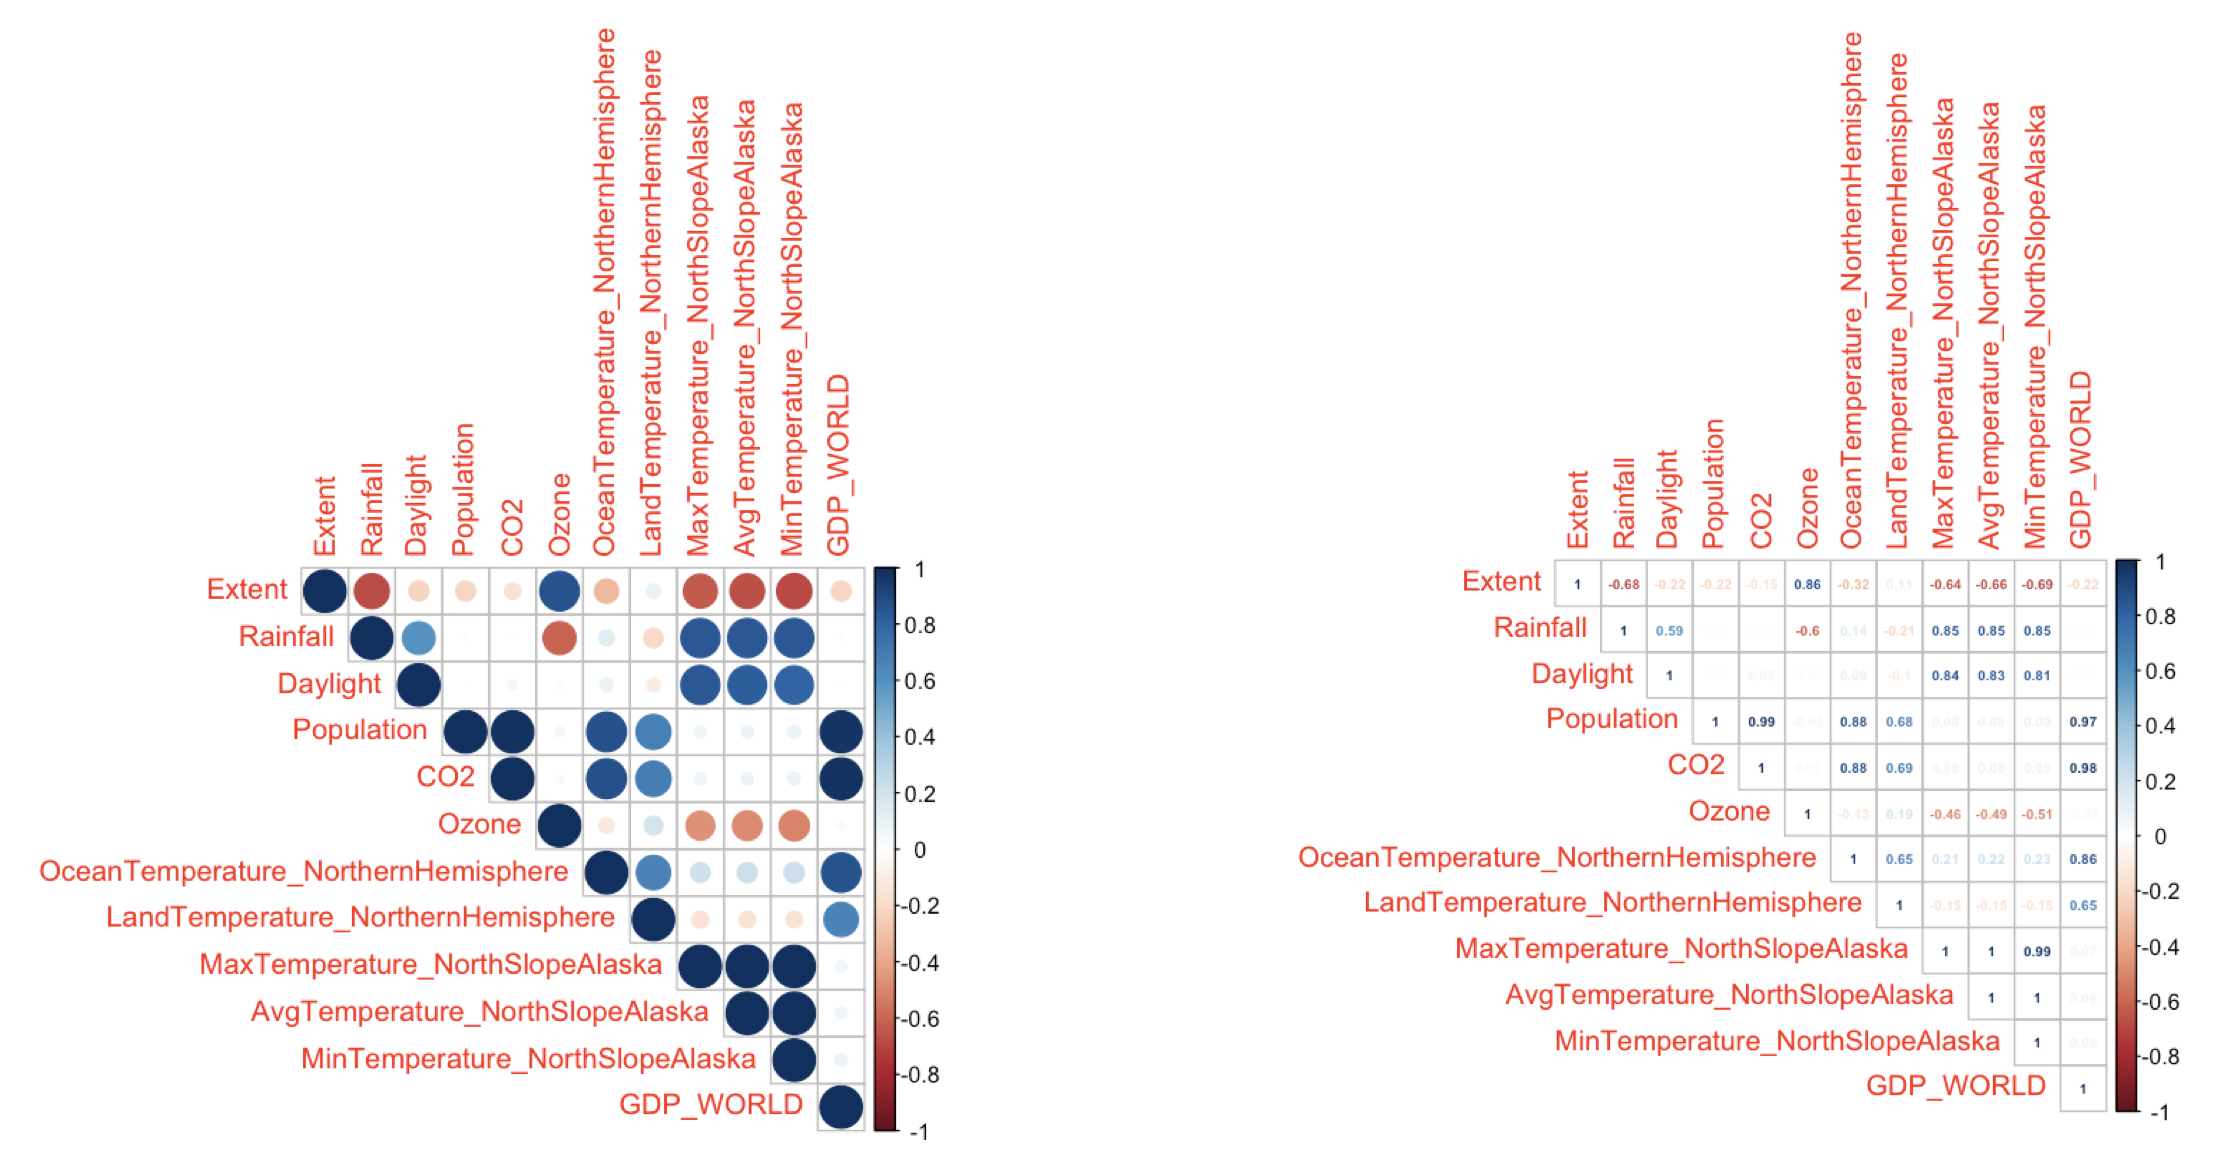
\includegraphics[width = 1.0\textwidth]{Figure/4.1-CM.png}
\caption{The correlation matrix of Arctic sea ice extent and rainfall in Alaska, Daylight in Alaska, Population of the World, the concentration of mid-tropospheric carbon dioxide, the minimum ozone found from total ozone satellite measurements north of 40°N, the ocean temperature in the Northern Hemisphere, the land temperature in the Northern Hemisphere, the maximum temperature of North Slope Alaska, the average temperature of North Slope Alaska, the minimum temperature of North Slope Alaska, the GDP of the World.}
\label{4.1-CM}
\end{figure}

\section{Sea Ice Now Forecasting} %4.2

\subsection{Linear Regression} %4.2.1

As the first algorithm, multiple Linear Regression model provides the most basic fitting results. Without the addition of penalty term, $\text{R}^2$ reached 0.8982 (as Figure \ref{4.2.1-LR-Training-Results} shows), but the mean square error reached 0.00946 when the test set was used for evaluation.

\begin{table}[htbp]
  \centering
  \footnotesize
  \begin{tabular}{p{5.75cm} | c c c c c c}
  \toprule
  Coefficients: \\ %row 1
    & Estimate & Std. Error & t value & $\text{Pr}(>|\text{t}|)$\\
  \hline
  (Intercept) & 0.72626 & 0.02602 & 27.912 & $< \text{2e-16}$ & ***\\
  Rainfall & 0.04478 & 0.02495 & 1.799 & 0.0727 & .\\
  Daylight & 0.18852 & 0.03376 & 5.583 & $\text{3.95e-08}$ & ***\\
  Population & -0.98423 & 0.13192 & -7.461 & $\text{4.07e-13}$ & ***\\
  CO2 & 1.86621 & 0.19379 & 9.630 & $< \text{2e-16}$ & ***\\
  Ozone & 0.39157 & 0.03262 & 12.003 & $< \text{2e-16}$ & ***\\
  OceanTemperature\_NorthernHemisphere & -0.23312 & 0.04408 & -5.289 & $< \text{1.87e-07}$ & ***\\
  LandTemperature\_NorthernHemisphere & 0.08561 & 0.03910 & 2.190 & 0.0290 & *\\
  MinTemperature\_NorthSlopeAlaska & -0.63691 & 0.05038 & -12.642 & $< \text{2e-16}$ & ***\\
  GDP\_WORLD & -69403 & 0.07102 & -9.772 & $< \text{2e-16}$ & ***\\
  \hline
  \multicolumn{6}{l}{Signif. codes: 0 '***' 0.001 '**' 0.01 '*' 0.05 '.' 0.1 '' 1} \\
  \multicolumn{6}{l}{Residual standard error: 0.08382 on 480 degrees of freedom}\\
  \multicolumn{6}{l}{   15894 observations deleted due to missingness}\\
  \multicolumn{6}{l}{Multiple R-squared: 0.8982,      Adjusted R-squared: 0.8963}\\
  \multicolumn{6}{l}{F-statistic: 470.5 on 9 and 480 DF, P-value: $< \text{2e-16}$}\\
  \bottomrule
  \end{tabular}
  \caption{Linear Regression training results.}
  \label{4.2.1-LR-Training-Results}
\end{table}



\begin{figure}[htbp]
\centering
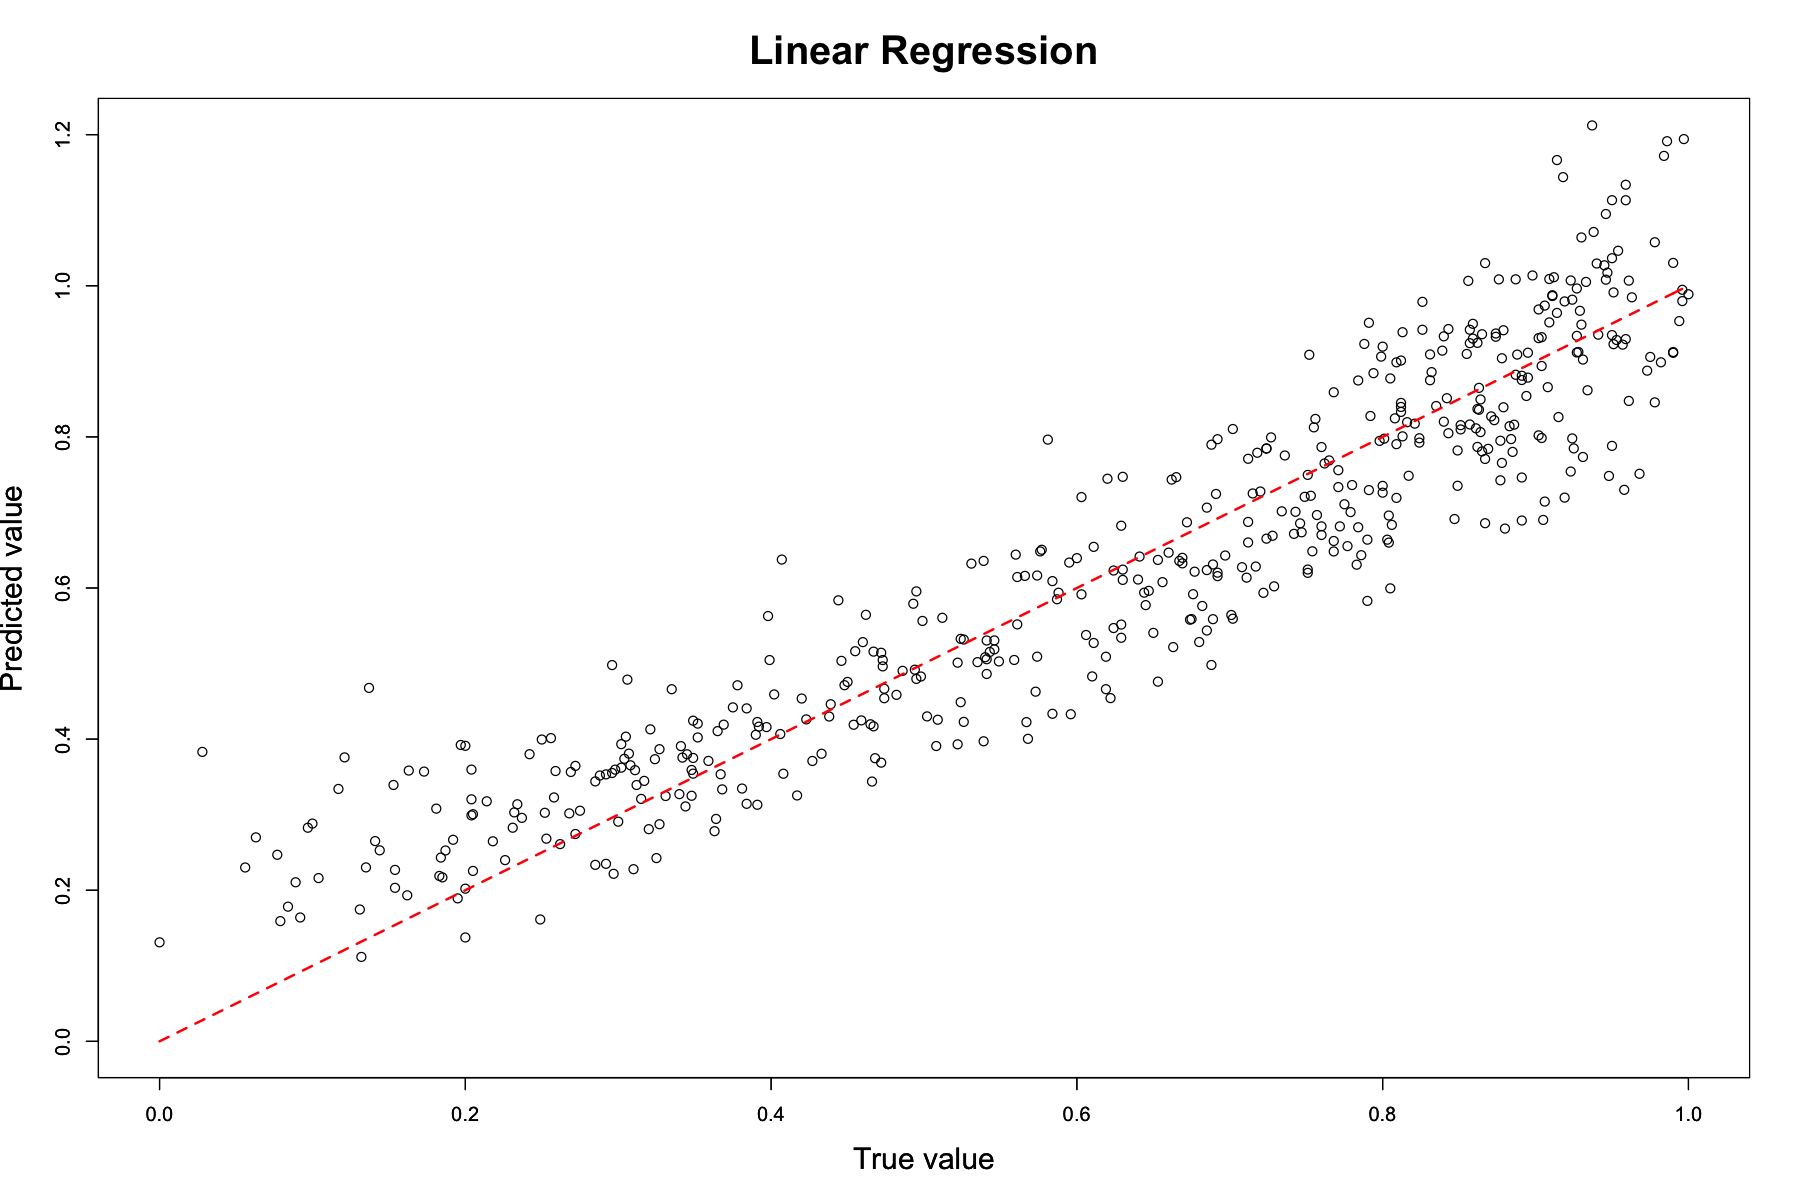
\includegraphics[width = 1.0\textwidth]{Figure/4.2.1-LR.png}
\caption{The predicted Arctic sea ice extent value vs the real Arctic sea ice extent value with Linear Regression. The red referenced dotted line represents the straight line y=x. Mean Square Error (MSE) is 0.00946.}
\label{4.2.1-LR}
\end{figure}


Using Figure \ref{4.2.1-LR}, it could be clearly found that the prediction result of Linear Regression has large error. In this case, a high $\text{R}^2$ corresponds to very poor test results. We guessed that there was an overfitting problem in the model, so we added a penalty term in the following training.



\subsection{Penalised Linear Regression (Lasso, min/1se)} %4.2.2

In order to simplify the model (reduce the number of features) while increasing the accuracy, Lasso penalization was applied on Penalized Linear Regression. Using the “glmnet” package, the weight of all features was drawn with the change of Lambda value. As the ridge-trance figure (Figure \ref{4.2.2-NEW-PLR-ridge-trance-Log-Lambda}) shows, as Lambda is worth increasing, more and more of the weights go to 0. Lasso Penalization is also based on this feature, when the Lambda increases, the feature with poor performance is gradually removed to realize the reduction of model complexity. 


\begin{figure}[htbp]
    \center
    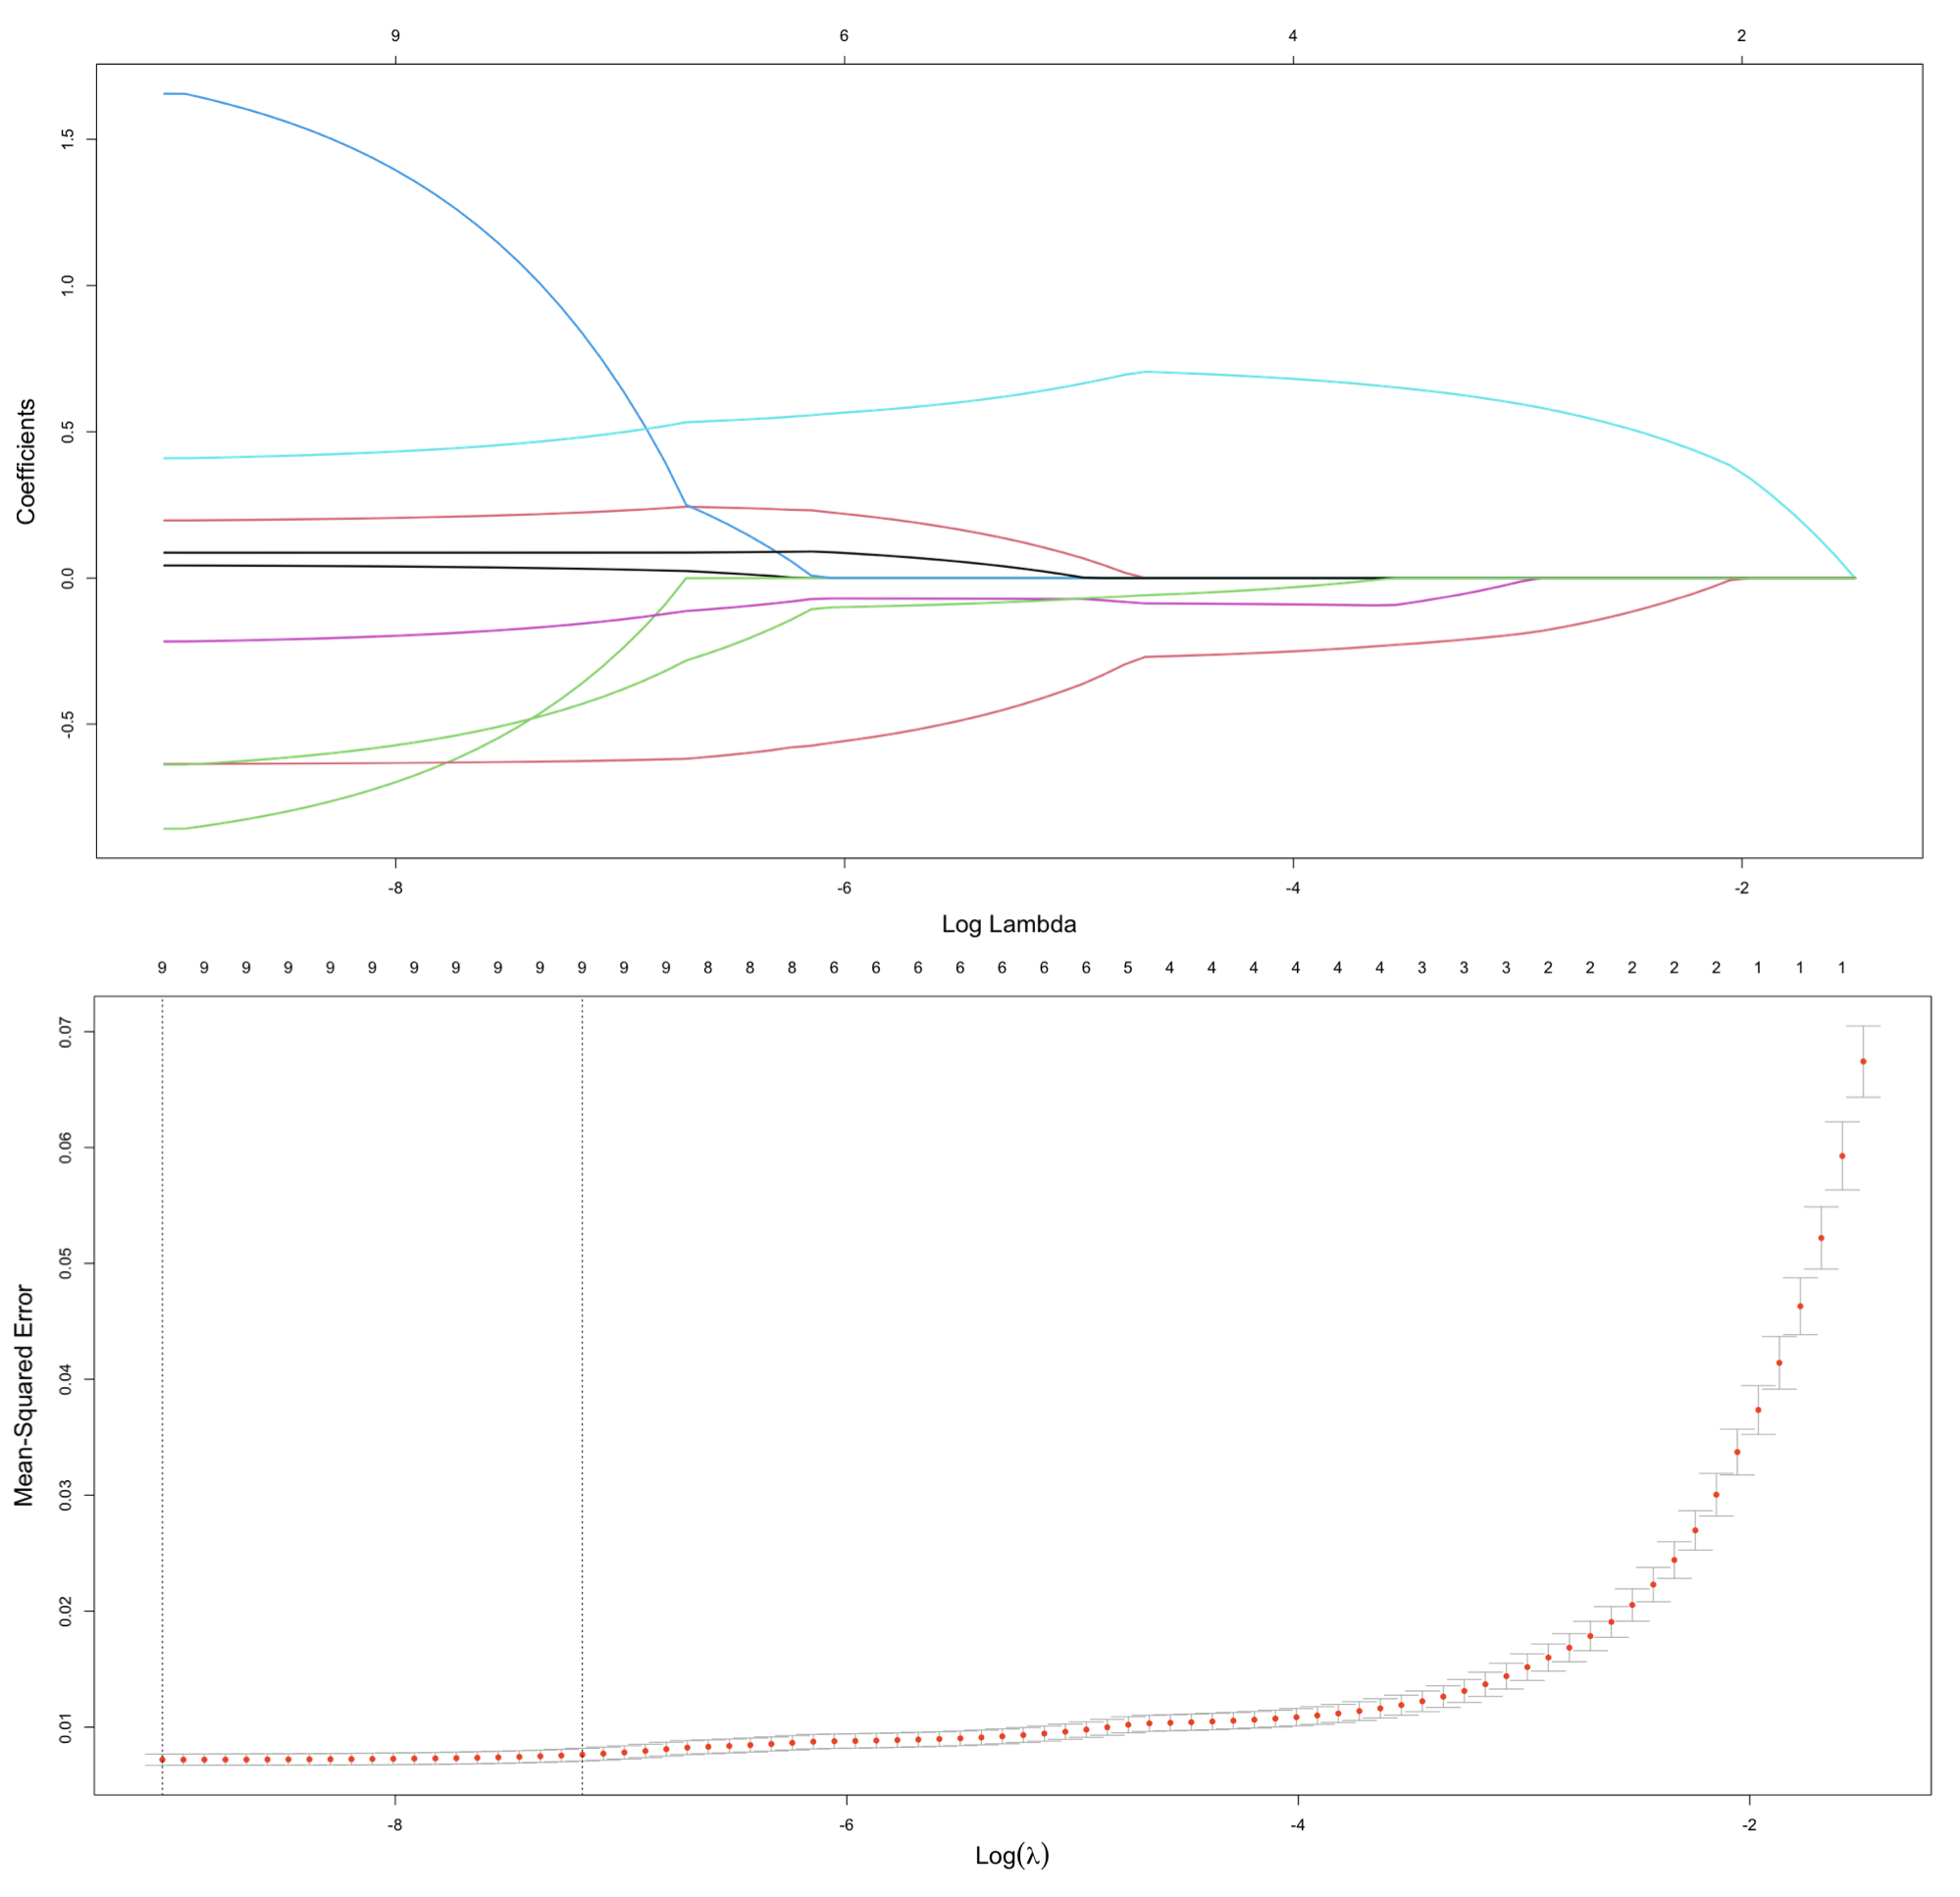
\includegraphics[scale=0.4]{Figure/4.2.2-NEW-PLR-ridge-trance-Log-Lambda.png}
    \caption{Top: Ridge trace diagram of Penalised Linear Regression; Bottom: Log Lambda vs Testing Error diagram of Penalised Linear Regression}
    \label{4.2.2-NEW-PLR-ridge-trance-Log-Lambda}
\end{figure}

%\begin{figure}[htbp]
%\centering
%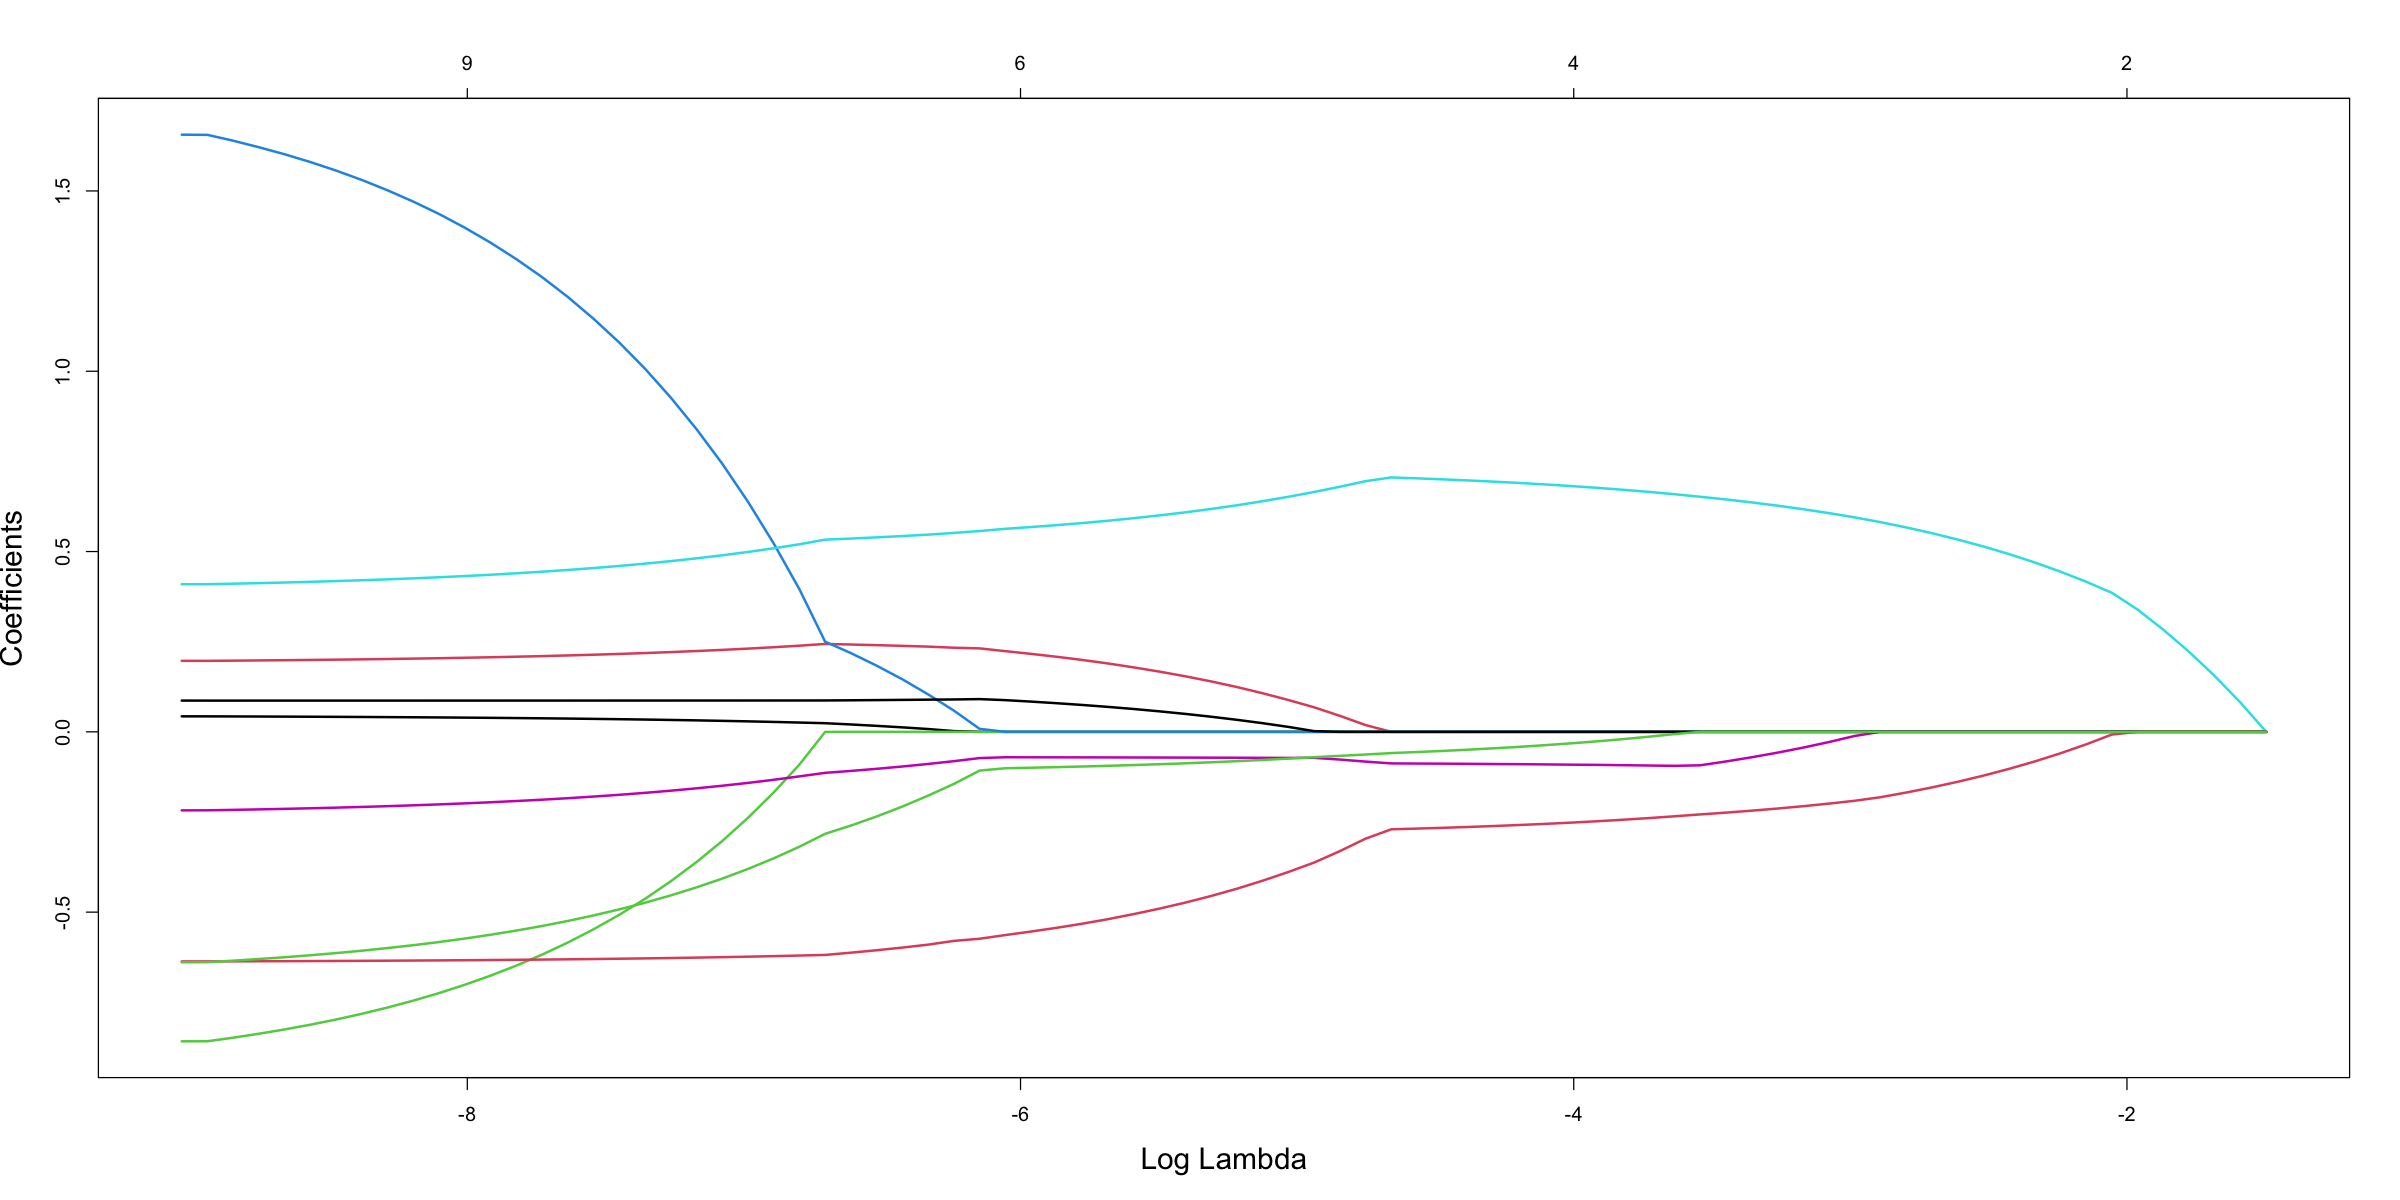
\includegraphics[width = 1.0\textwidth]{Figure/4.2.2-PLR-ridge-trance.png}
%\caption{Ridge trace diagram of Penalised Linear Regression}
%\label{4.2.2-PLR-ridge-trance}
%\end{figure}

At this point, appropriate Lambda values were needed to be selected to output weights of all features. In the selection, min and 1se option were applied respectively (Such as the x value corresponding to the two dotted lines in following Figure \ref{4.2.2-NEW-PLR-ridge-trance-Log-Lambda}).

%\begin{figure}[htbp]
%\centering
%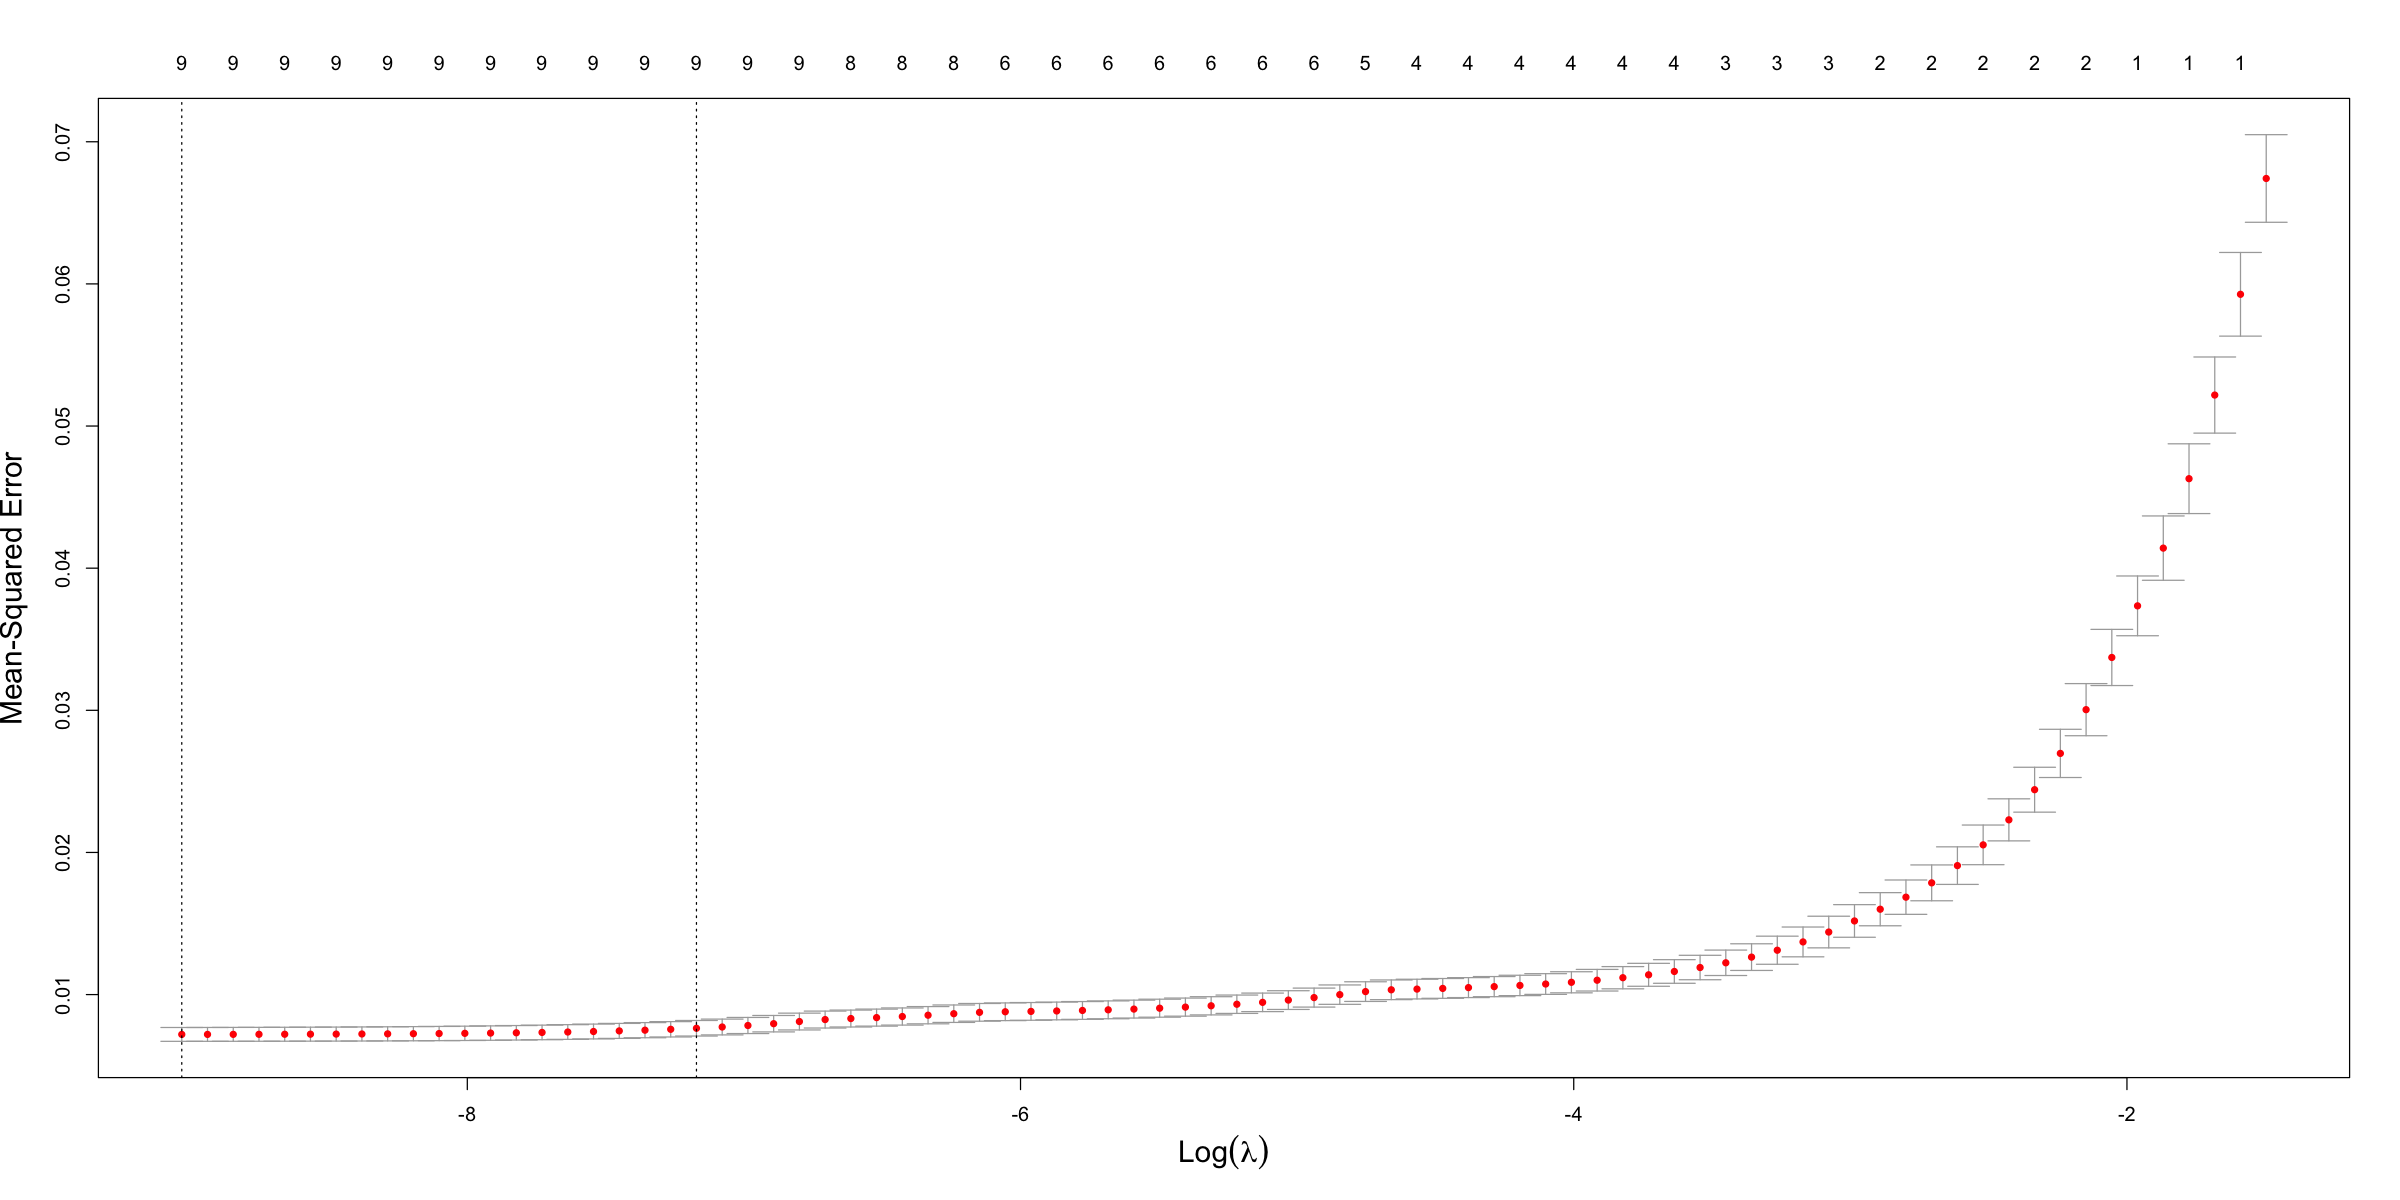
\includegraphics[width = 1.0\textwidth]{Figure/4.2.2-PLR-Log-Lambda-vs-Testing-Error.png}
%\caption{Log Lambda vs Testing Error diagram of Penalised Linear %Regression}
%\label{4.2.2-PLR-Log-Lambda-vs-Testing-Error}
%\end{figure}

Applying different option of Lambda value, two different sets of results were obtained. When Lambda option is min, the MSE value of the model is 0.00690, which is slightly less than the 0.00734 that obtained when Lambda option is 1se. The output result is shown in following Table \ref{4.2.2-PLR-para}. In this case, using 1se will not reduce the complexity of the model (reduce the number of features) but it will lose the accuracy. Therefore, in this Lasso Regression, min value is the better choice for Lambda.

\begin{table}[t]
  \centering
  \footnotesize
  \begin{tabular}{p{5.75cm} | r | r}
  \toprule
  Coefficients: & min & 1se\\ %row 1
  \hline
    & 1 & 1\\
  (Intercept) & 0.71559335 & 0.66666336\\
  Rainfall & 0.04299020 & 0.03049067\\
  Daylight & 0.19686230 & 0.22725958\\
  Population & -0.85828586 & -0.30290499\\
  CO2 & 1.65605218 & 0.74378027\\
  Ozone & 0.40941811 & 0.48953790\\
  OceanTemperature\_NorthernHemisphere & -0.21778615 & -0.14950798\\
  LandTemperature\_NorthernHemisphere & 0.08669526 & 0.08684475\\
  MinTemperature\_NorthSlopeAlaska & -0.63667606 & -0.62486026\\
  GDP\_WORLD & -0.63894945 & -0.40706240\\
  \bottomrule
  \end{tabular}
  \caption{Hyper-parameters of Penalised Linear Regression.}
  \label{4.2.2-PLR-para}
\end{table}


In terms of fitting, the performance of the two (applying min, 1se value of Lambda) are general and basically the same. Compared with the normal Linear Regression before the penalty term was applied, the performance of the test fitting is optimized but still not ideal. This is due to the lack of flexibility in the model.


\begin{figure}[htbp]
\centering
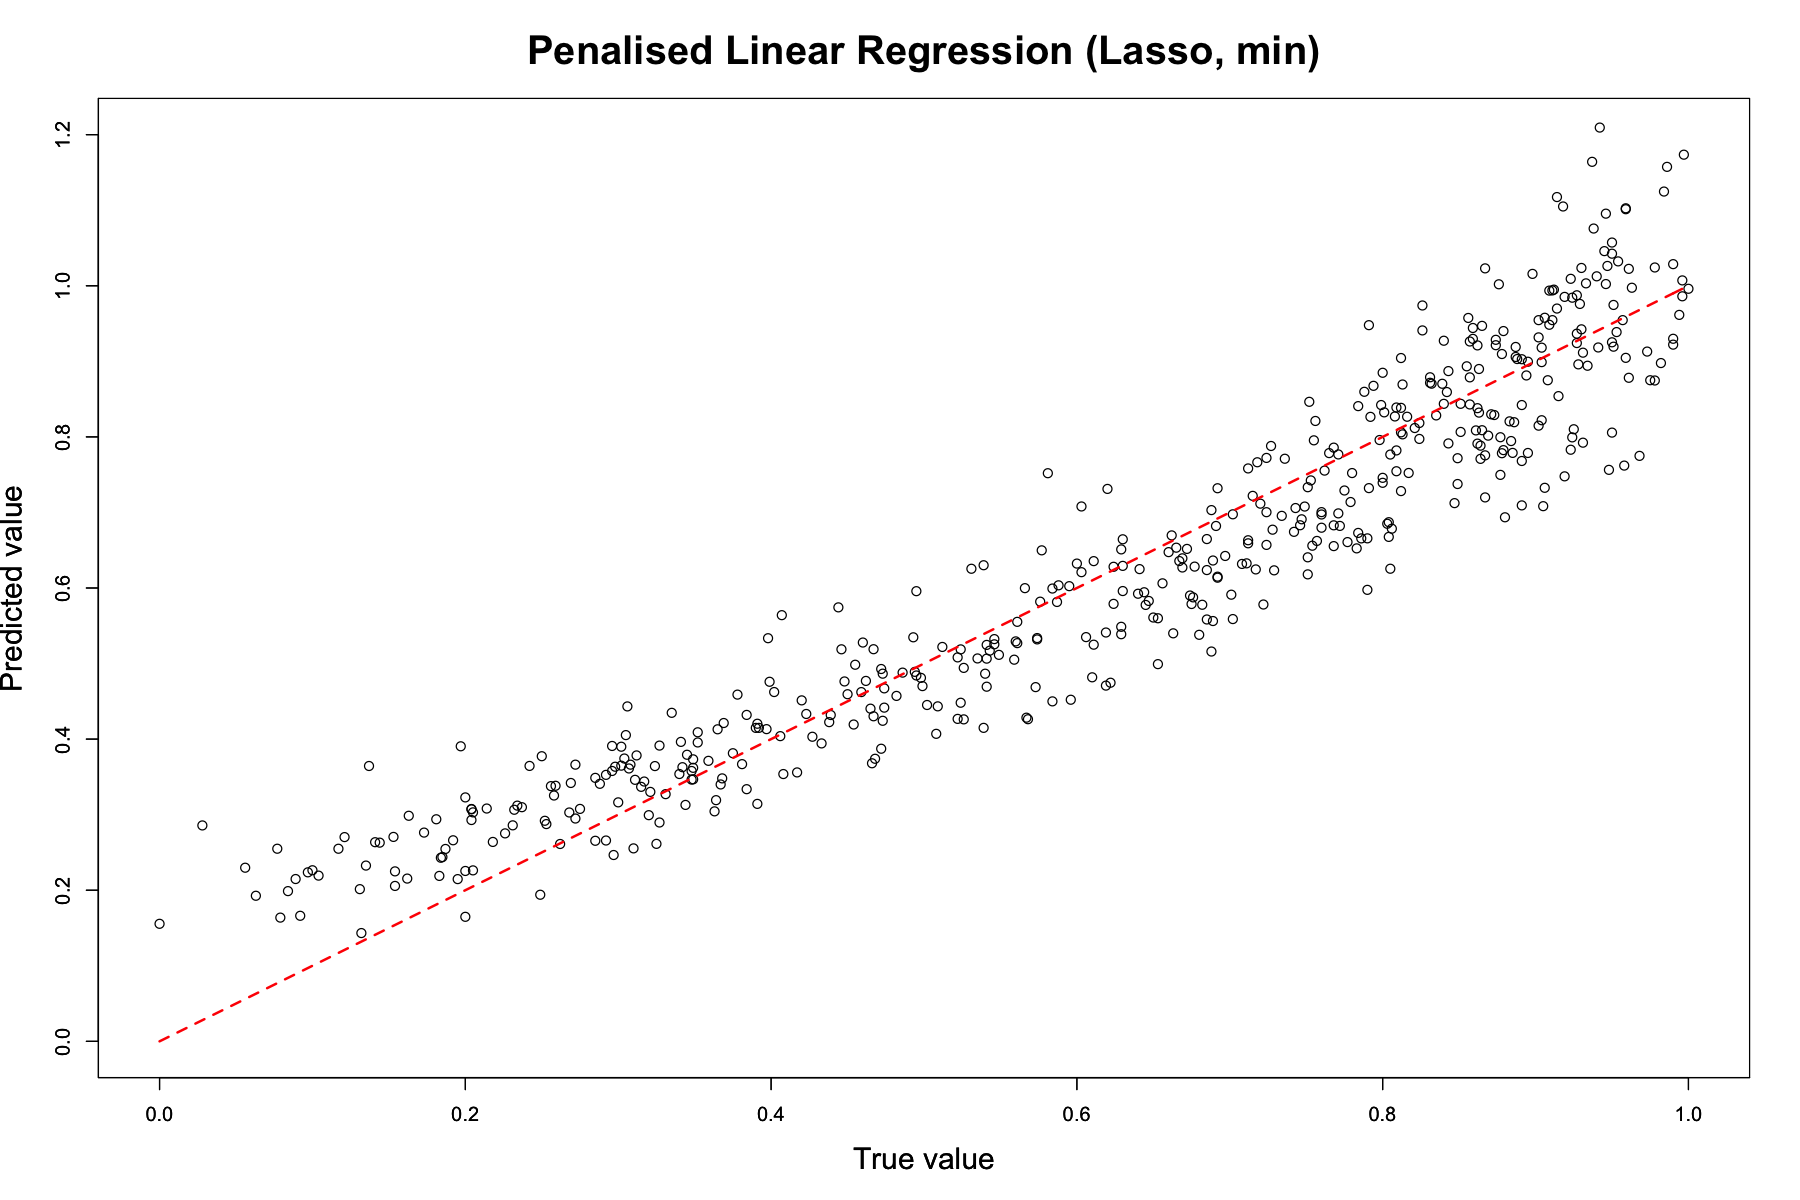
\includegraphics[width = 1.0\textwidth]{Figure/4.2.2-PLR-min.png}
\caption{The predicted Arctic sea ice extent value vs the real Arctic sea ice extent value with Penalised Linear Regression (Lasso, min). The red referenced dotted line represents the straight line y=x. Mean Square Error (MSE) is 0.00690.}
\label{4.2.2-PLR-min}
\end{figure}


\begin{figure}[htbp]
\centering
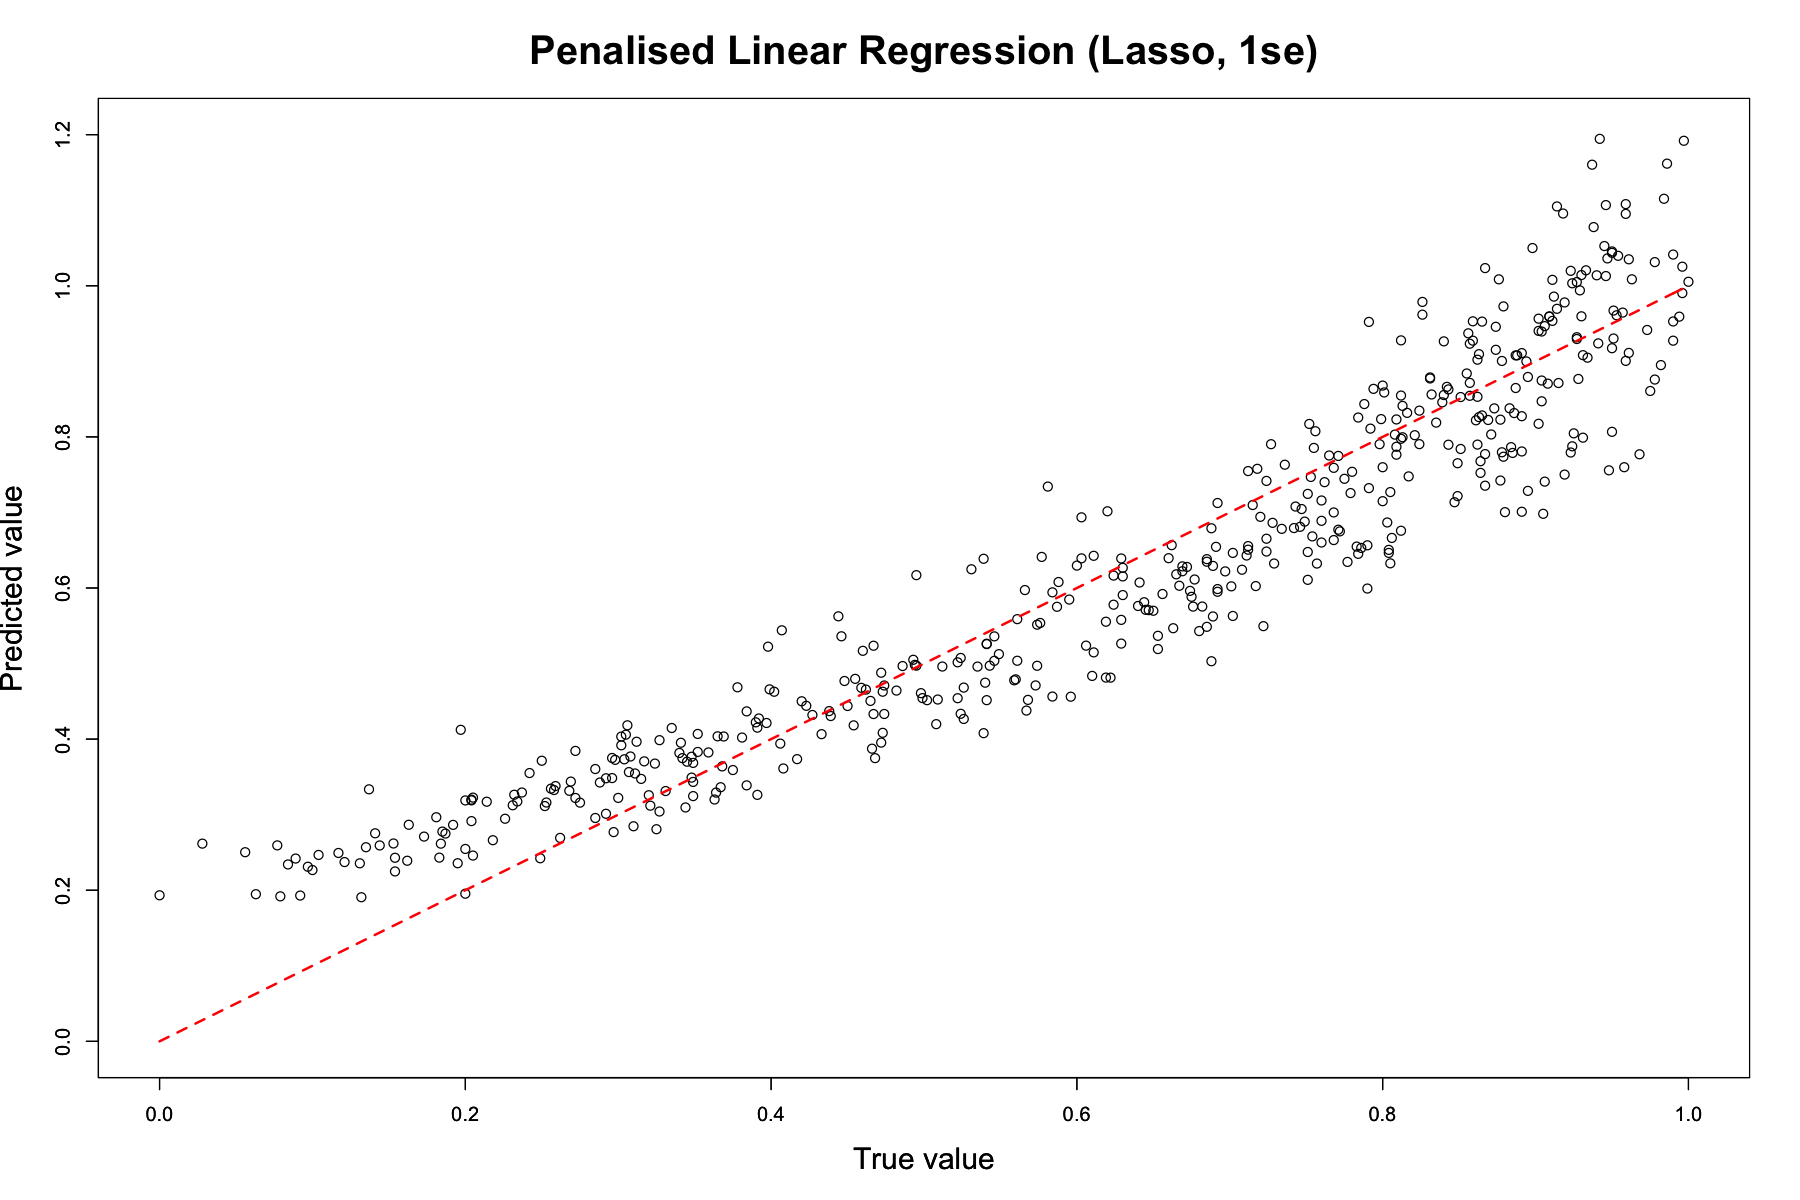
\includegraphics[width = 1.0\textwidth]{Figure/4.2.2-PLR-1se.png}
\caption{The predicted Arctic sea ice extent value vs the real Arctic sea ice extent value with Penalised Linear Regression (Lasso, 1se). The red referenced dotted line represents the straight line y=x. Mean Square Error (MSE) is 0.00732.}
\label{4.2.2-PLR-1se}
\end{figure}



\subsection{Penalised Polynomial Regression (Lasso, min/1se)} %4.2.3
To increase the flexibility of the model, polynomial regression was applied. Based on the correlation matrix, the four features with the best correlation were selected for this model. The order of one to four of each feature was added to the training. Similarly, polynomial regression suffered from overfitting, so the Lasso penalty term was still used in this model.

Again, ridge-trance graph was generated.

Similarly, applying log Lambda vs testing error **GRAPH**, the Lambda value can be chosen.

According to the following **RESULTS (the table)**, it can be seen that all the features (16) are kept in this model applying min Lambda value while only 10 features are kept applying 1se. In this case, unlike the previous Penalized Linear Regression, applying 1se value of Lambda achieve cancelling nearly half of the features, which is able to greatly simplifies the model. Comparing the MSE of both options, MSE equals to 0.00448 when min value is applied. In comparison, the MSE only increases to 0.00483 applying 1se. At the cost of small precision loss, the model can be greatly simplified, which is exactly the purpose of the 1se option of Lambda.

By comparing the fitting **DIAGRAM** of two results, it can be found that the results are similar, which further proves that the influence of 1se value on the accuracy of the model is almost negligible. At the same time, compared with linear regression, the fitting results were significantly better, which was due to the fact that polynomial regression brought more flexibility to the model.



\begin{figure}[htbp]
    \center
    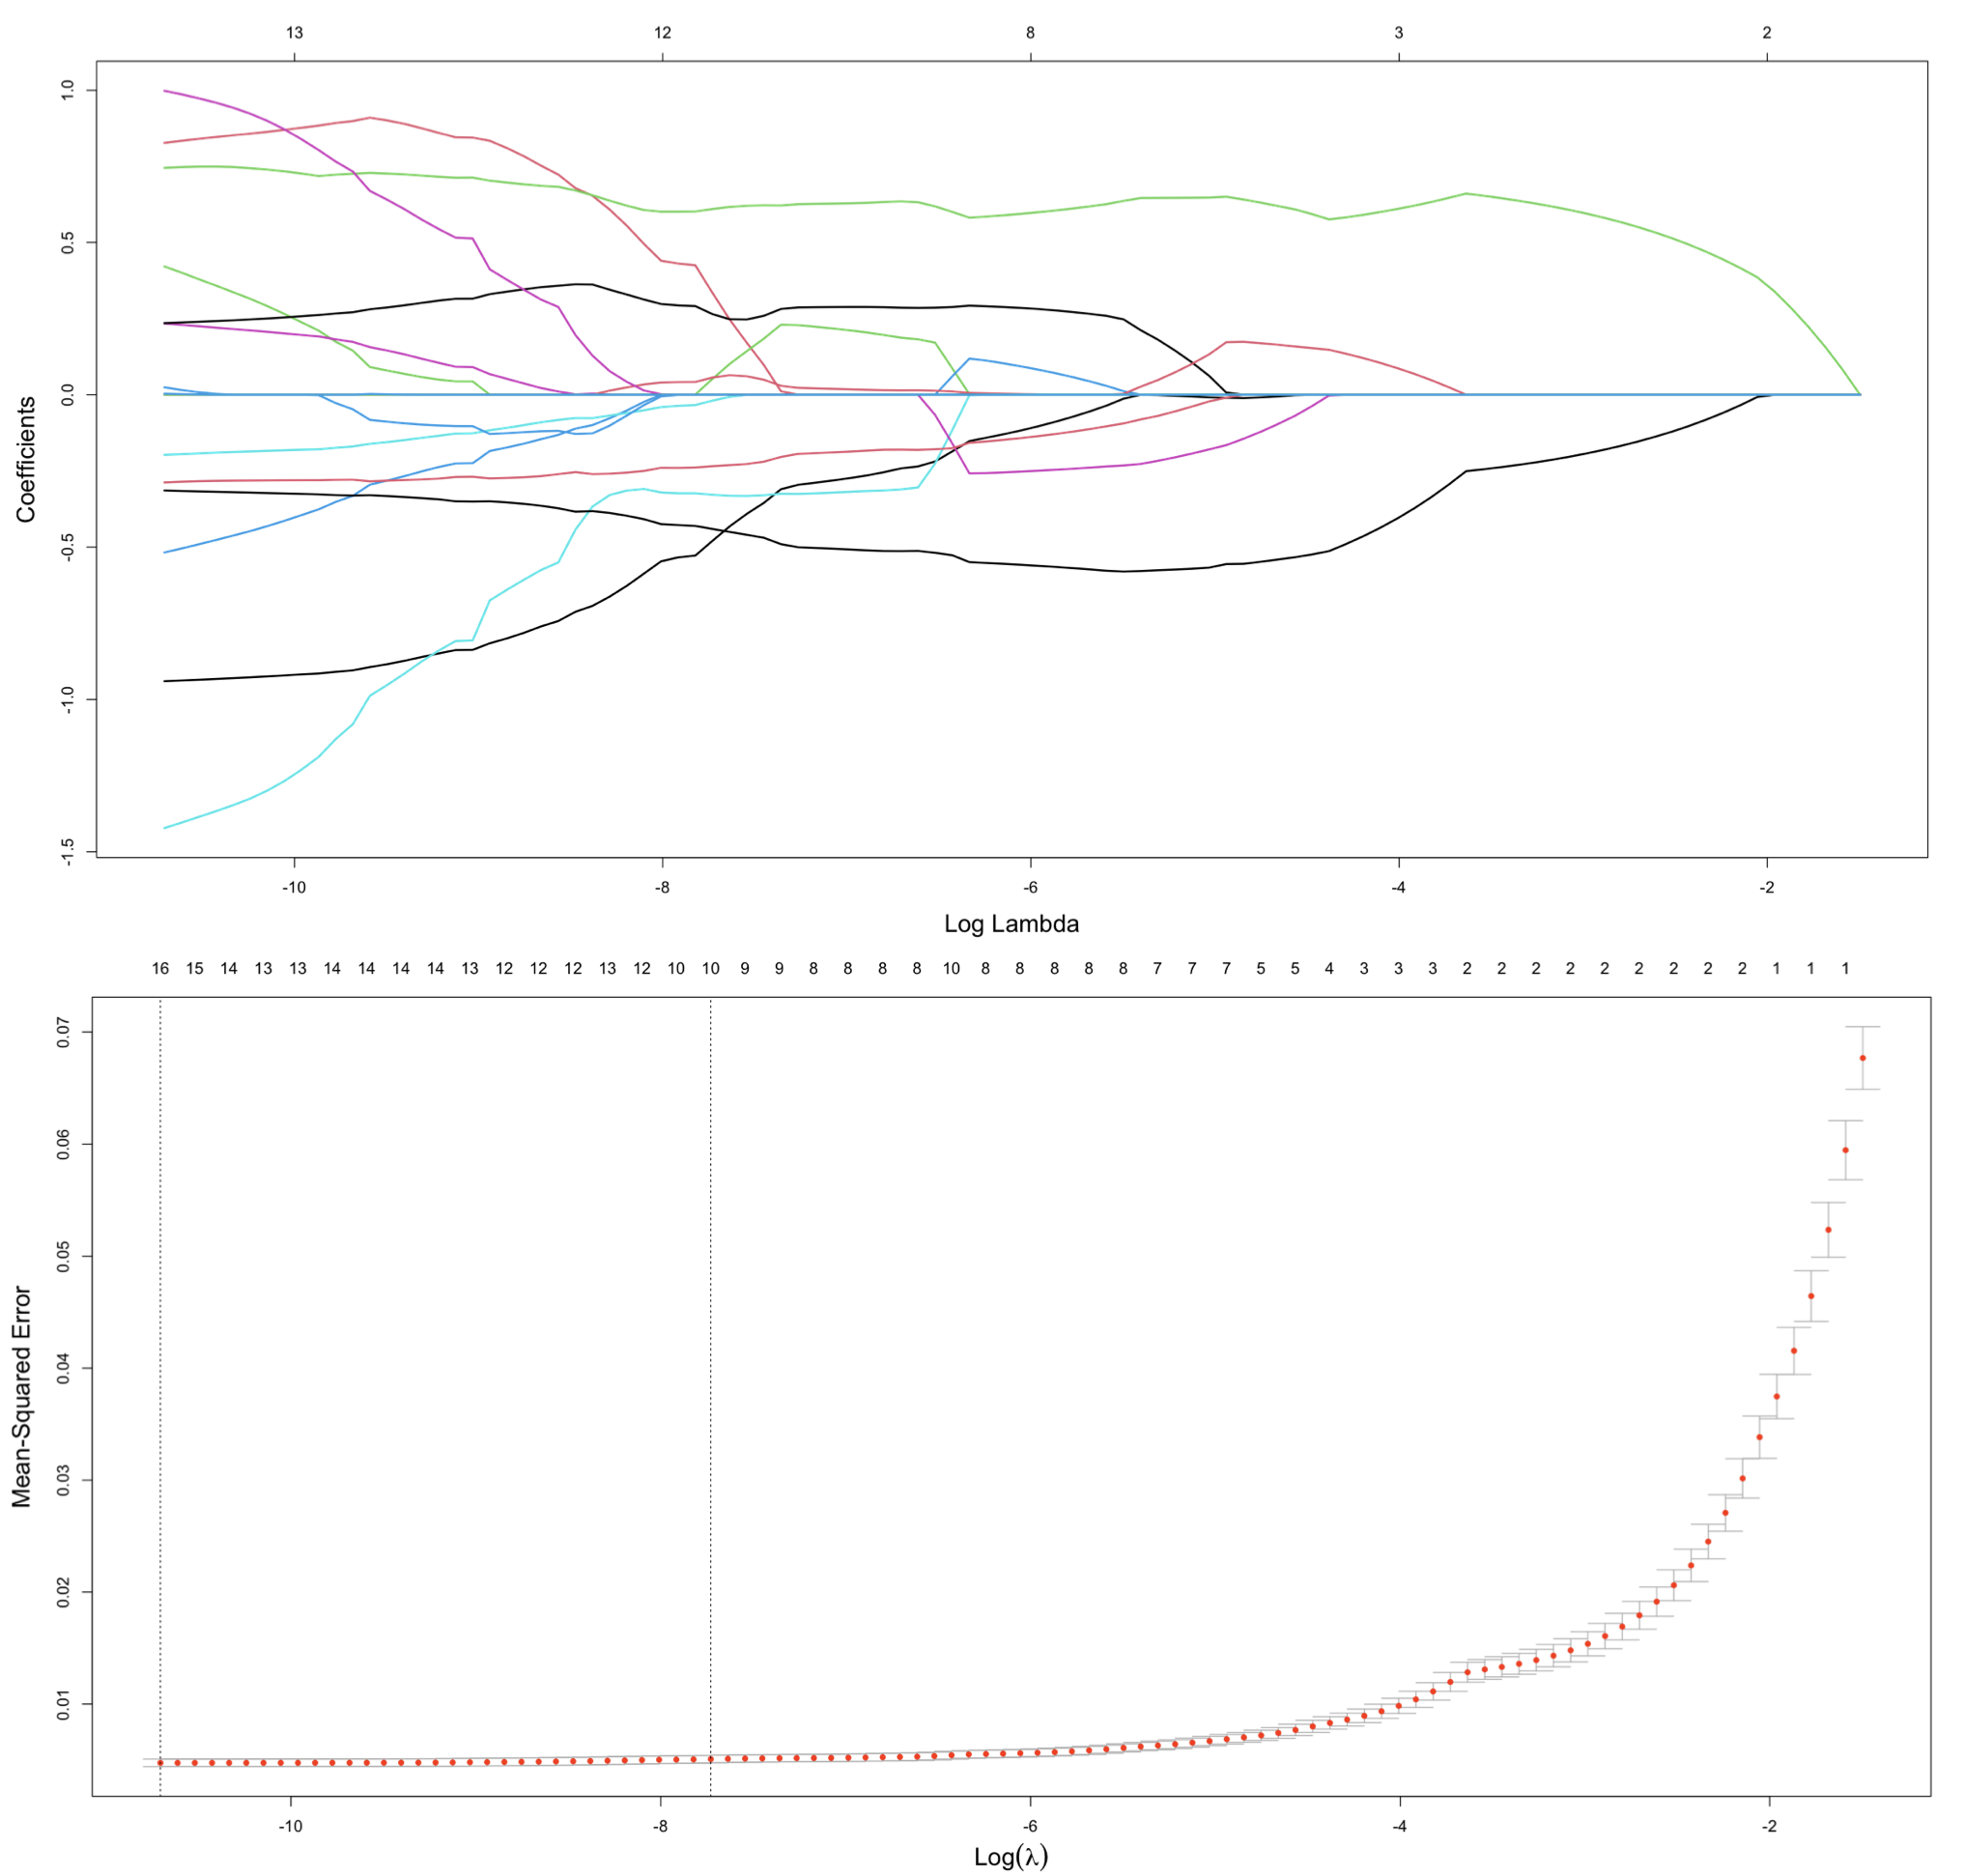
\includegraphics[scale=0.4]{Figure/4.2.3-NEW-PPR-ridge-trance-Log-Lambda.png}
    \caption{Top: Ridge trace diagram of Penalised Polynomial Regression; Bottom: Log Lambda vs Testing Error diagram of Penalised Polynomial Regression}
    \label{4.2.3-NEW-PPR-ridge-trance-Log-Lambda}
\end{figure}


\begin{figure}[htbp]
\centering
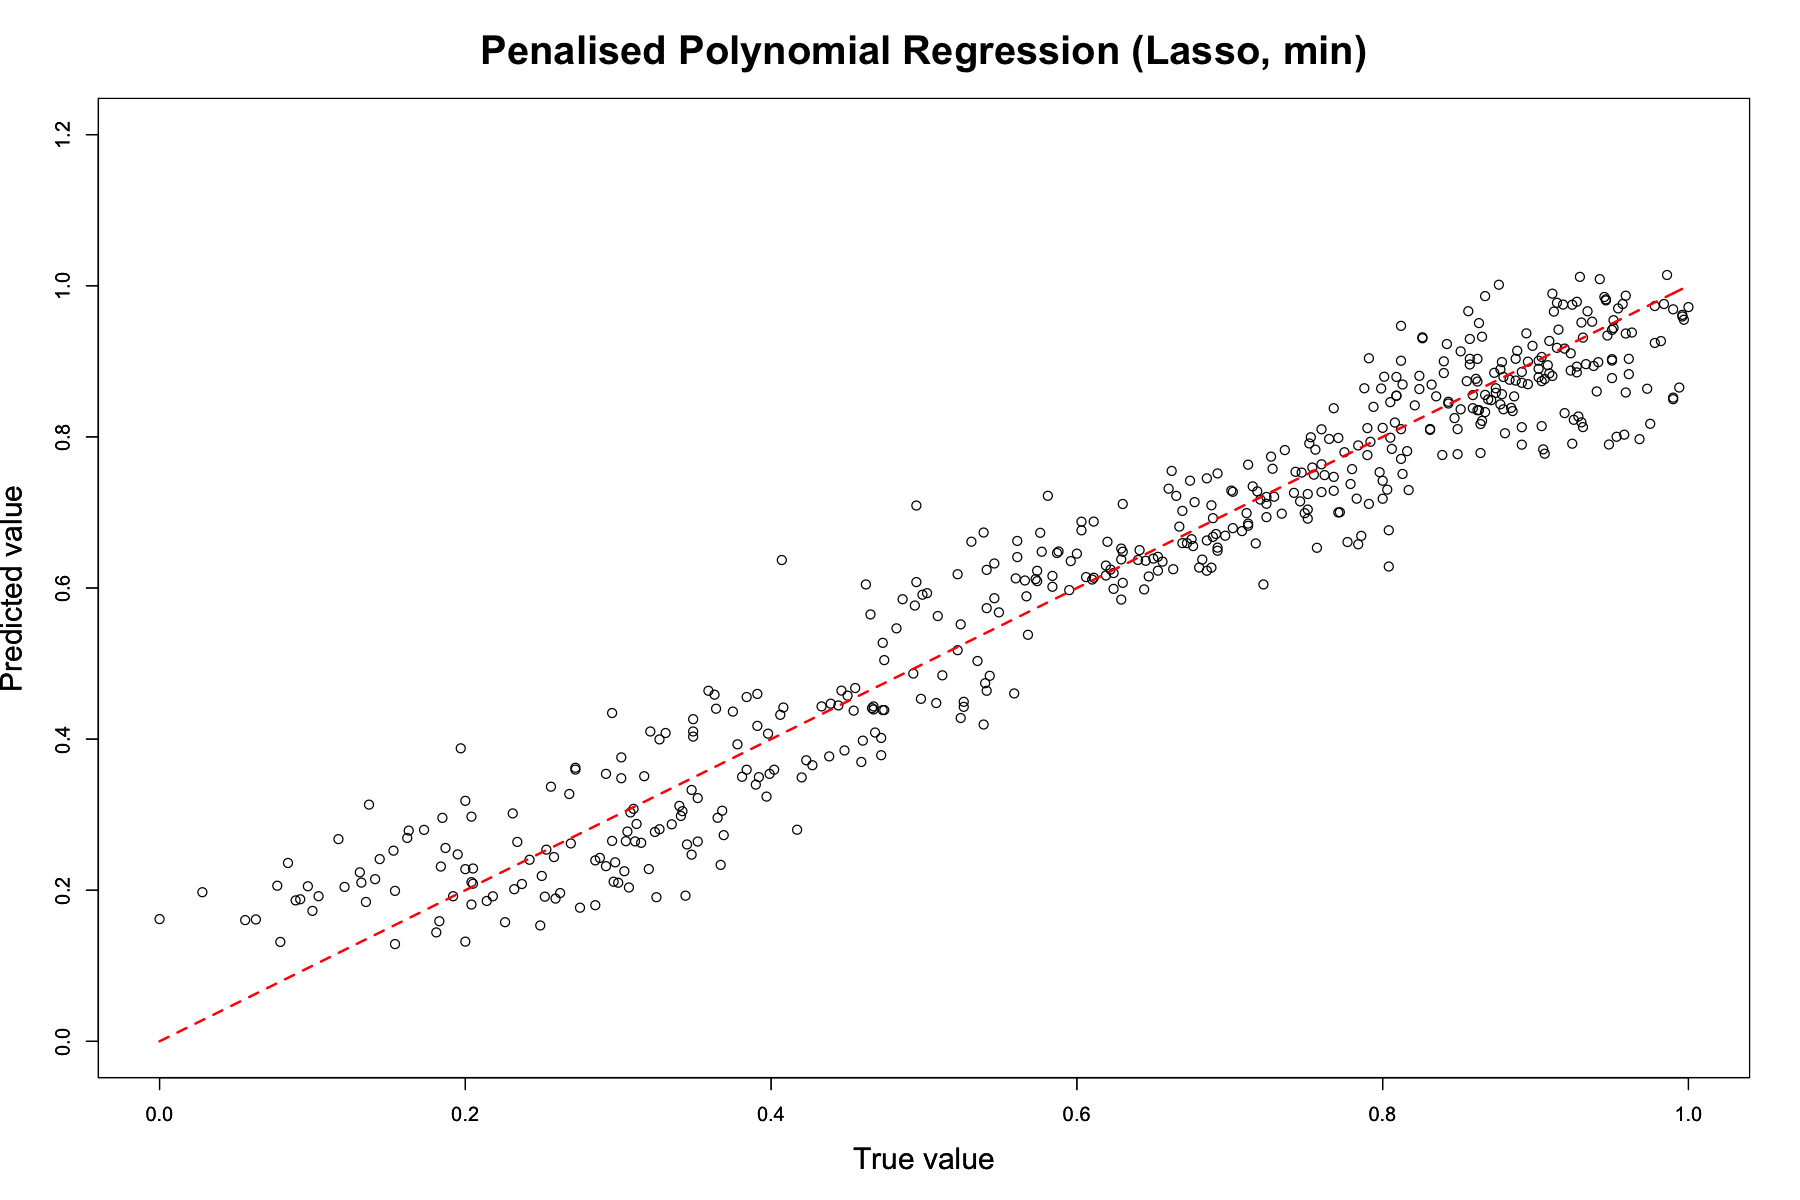
\includegraphics[width = 1.0\textwidth]{Figure/4.2.3-PPR-min.png}
\caption{The predicted Arctic sea ice extent value vs the real Arctic sea ice extent value with Penalised Polynomial Regression (Lasso, min). The red referenced dotted line represents the straight line y=x. Mean Square Error (MSE) is 0.00448.}
\label{4.2.3-PPR-min}
\end{figure}

\begin{figure}[htbp]
\centering
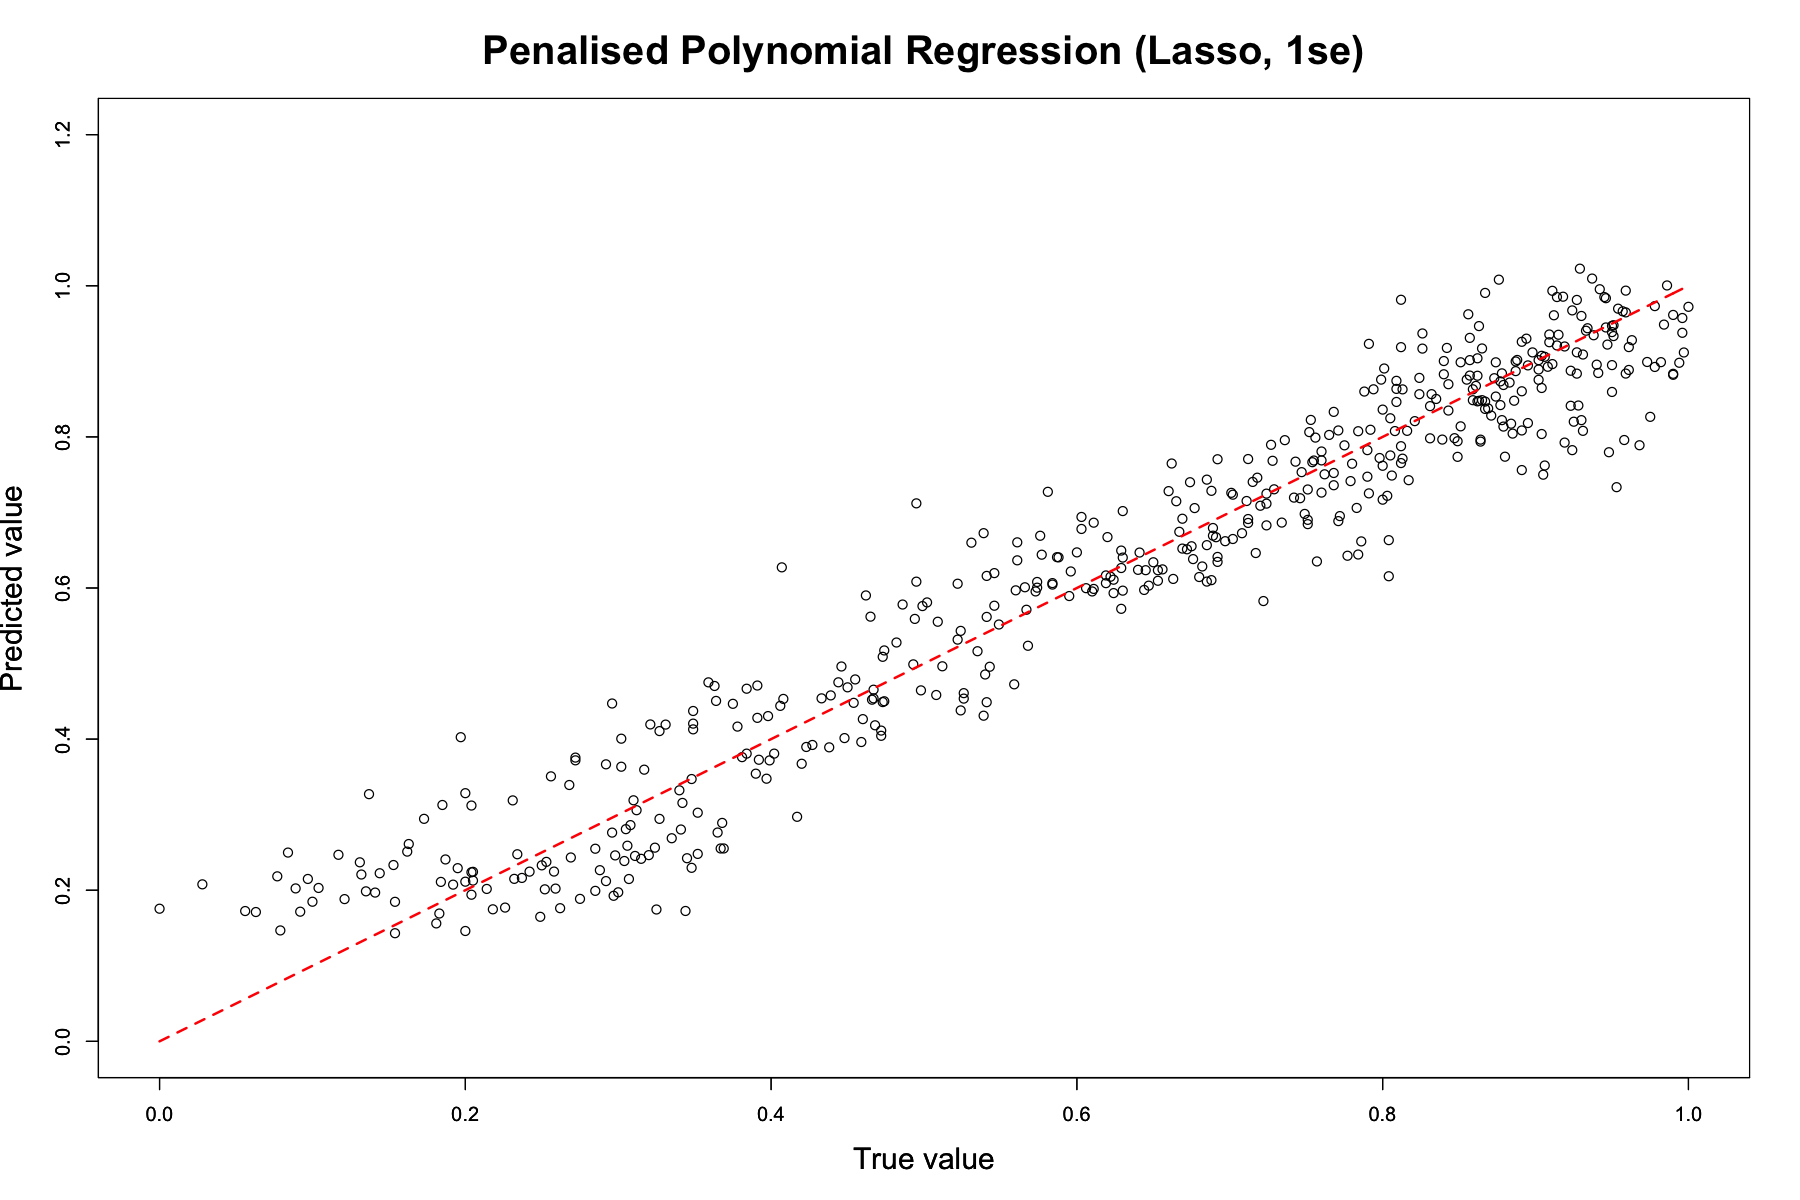
\includegraphics[width = 1.0\textwidth]{Figure/4.2.3-PPR-1se.png}
\caption{The predicted Arctic sea ice extent value vs the real Arctic sea ice extent value with Penalised Polynomial Regression (Lasso, 1se). The red referenced dotted line represents the straight line y=x. Mean Square Error (MSE) is 0.00484.}
\label{4.2.3-PPR-1se}
\end{figure}



\subsection{Random Forest} %4.2.4

To use Random Forest, three parameters need to be determined, namely, the number of total features, the number of trees, and mtry (number of features that randomly applied in each tree). Firstly, 9 out of 11 features are applied in this algorithm based on correlation matrix. Then, the “tree number vs out-of-bag error” graph (Figure \ref{4.2.6-RF-200TreesStable}) was plotted. It can be seen that, based on different mtry values, when the tree number approaches 200, the out-of-bag error tends to be stable. Therefore, 200 is chosen as the tree number of this model.

\begin{figure}[htbp]
\centering
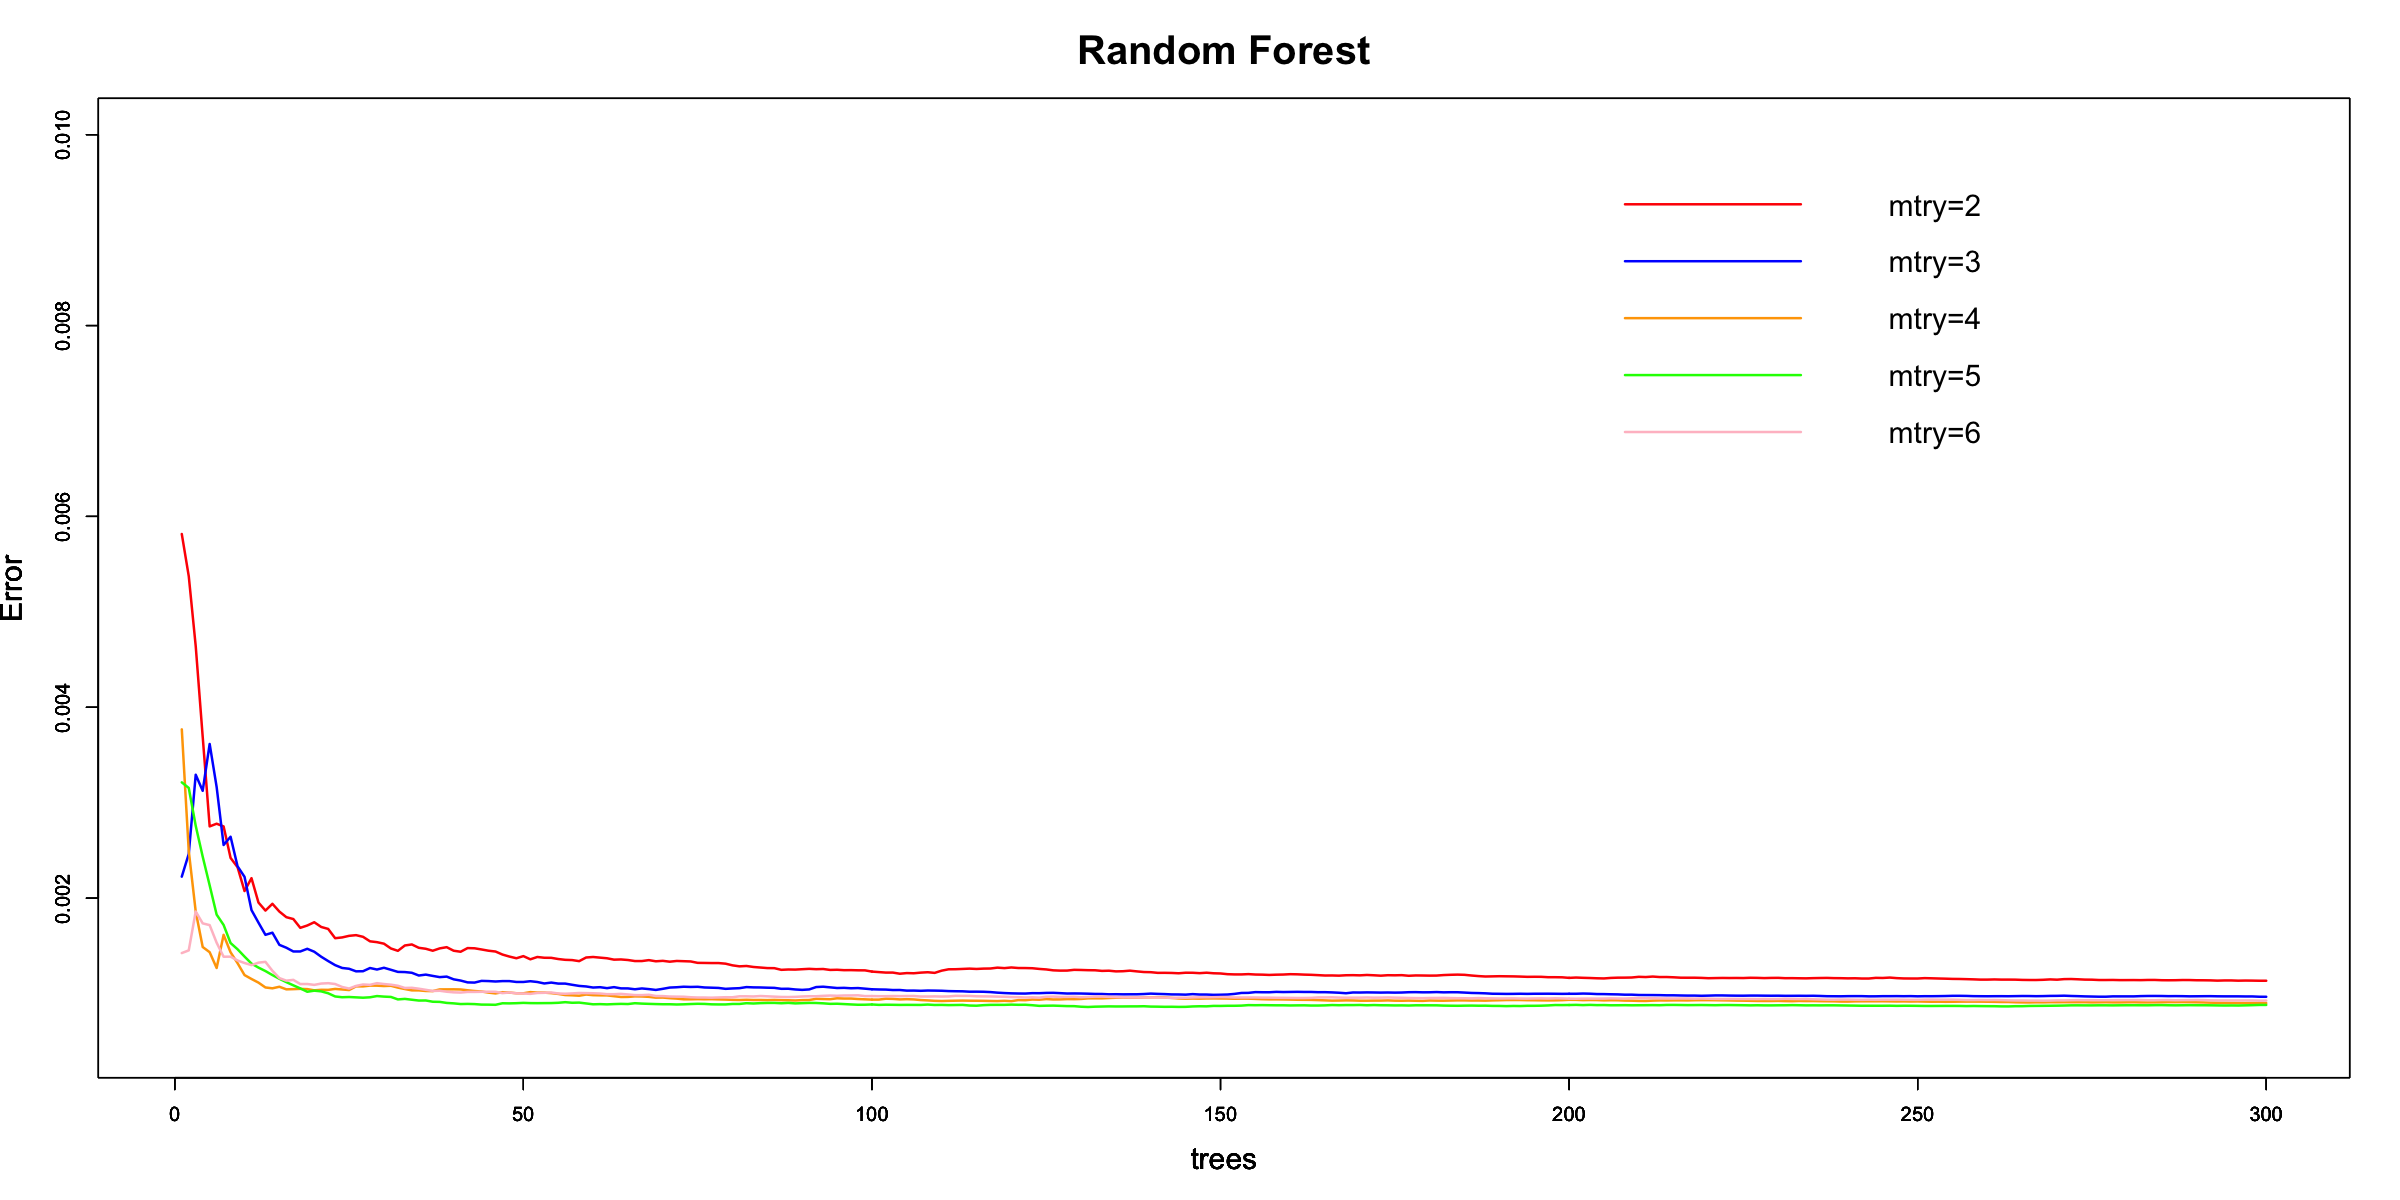
\includegraphics[width = 1.0\textwidth]{Figure/4.2.4-RF-200TreesStable.png}
\caption{Check the error stability of random forest with different number of trees.}
\label{4.2.6-RF-200TreesStable}
\end{figure}

Moreover, the choice of the mtry value is also important. Based on the already selected tree number 200. By using different mtry (from 2-6) values training models, different out-of-bag errors will be obtained. Through comparison, 5 is finally selected as mtry value, which corresponds with minimum out-of-bag error.

\begin{figure}[htbp]
\centering
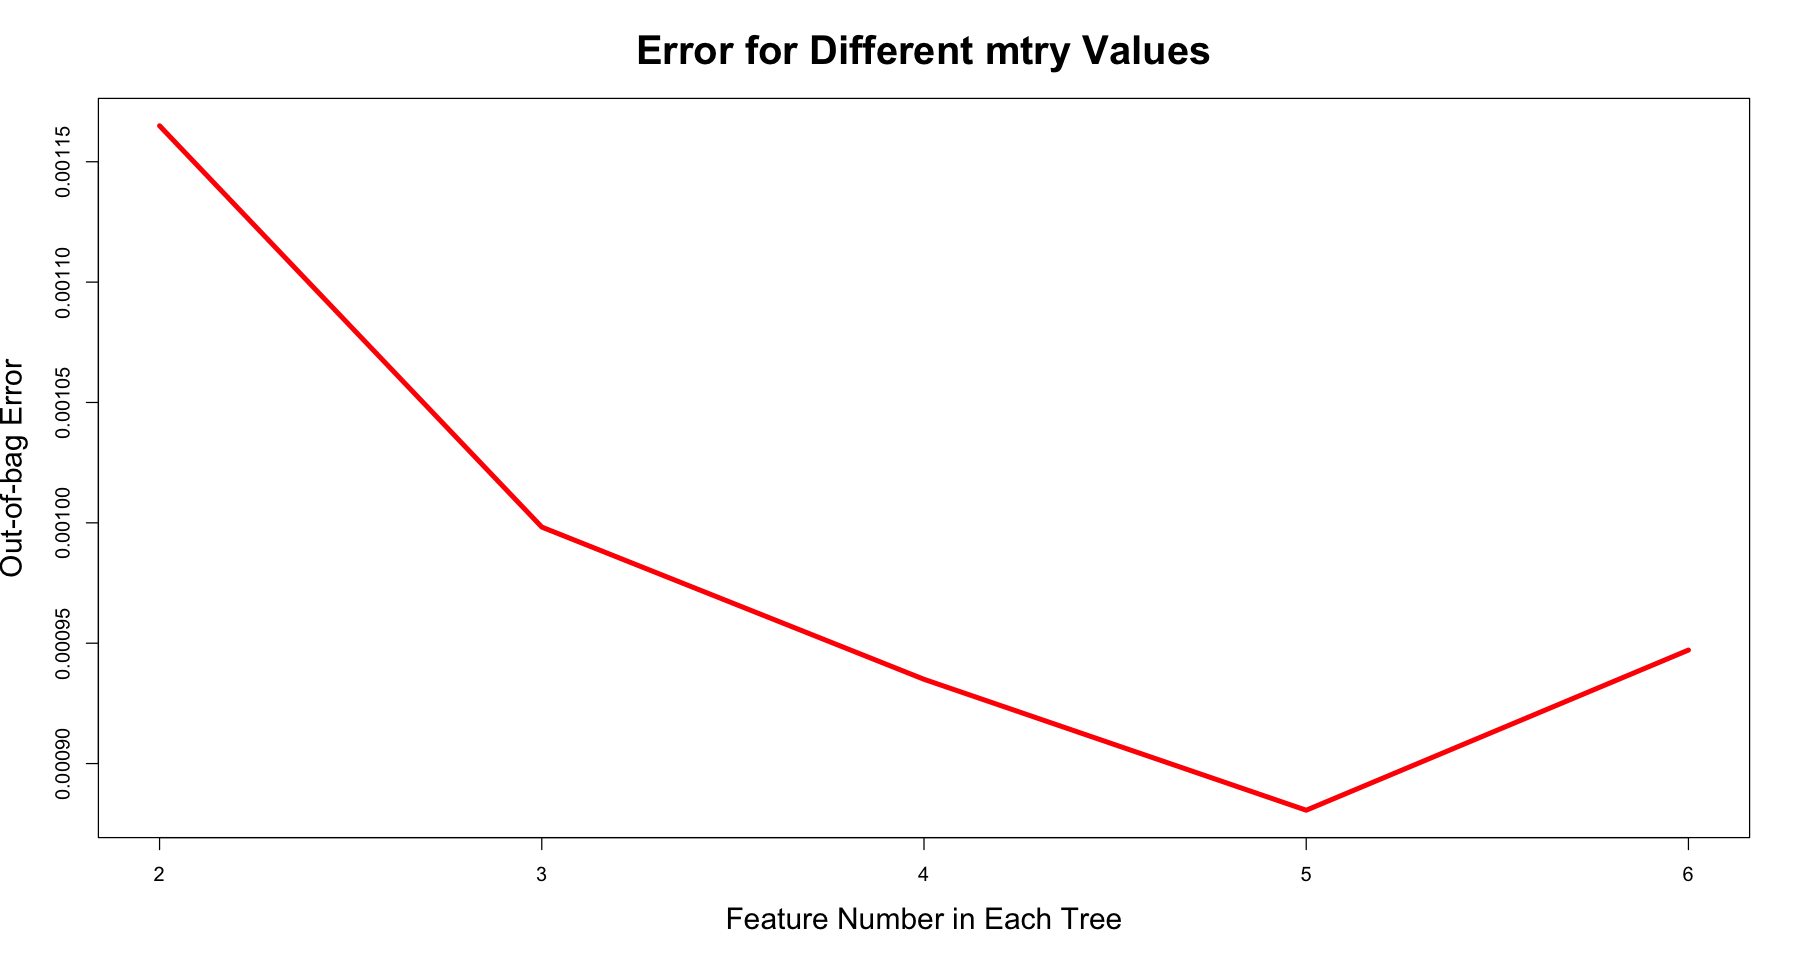
\includegraphics[width = 1.0\textwidth]{Figure/4.2.4-RF-5Features.png}
\caption{Check the out-of-bag error of random forest with different number of features in each tree when three number is 200.}
\label{4.2.4-RF-5Features}
\end{figure}

After Parameter selection, Random Forest model can be trained and tested. The MSE output is 0.00105, which is much lower than the previous models. Observing the fitting diagram (Figure \ref{4.2.4-RF}), it can be found that the dots are distributed in a narrow area fitting the straight line x=y, which indicated the performance of Random Forest is satisfying.

\begin{figure}[htbp]
\centering
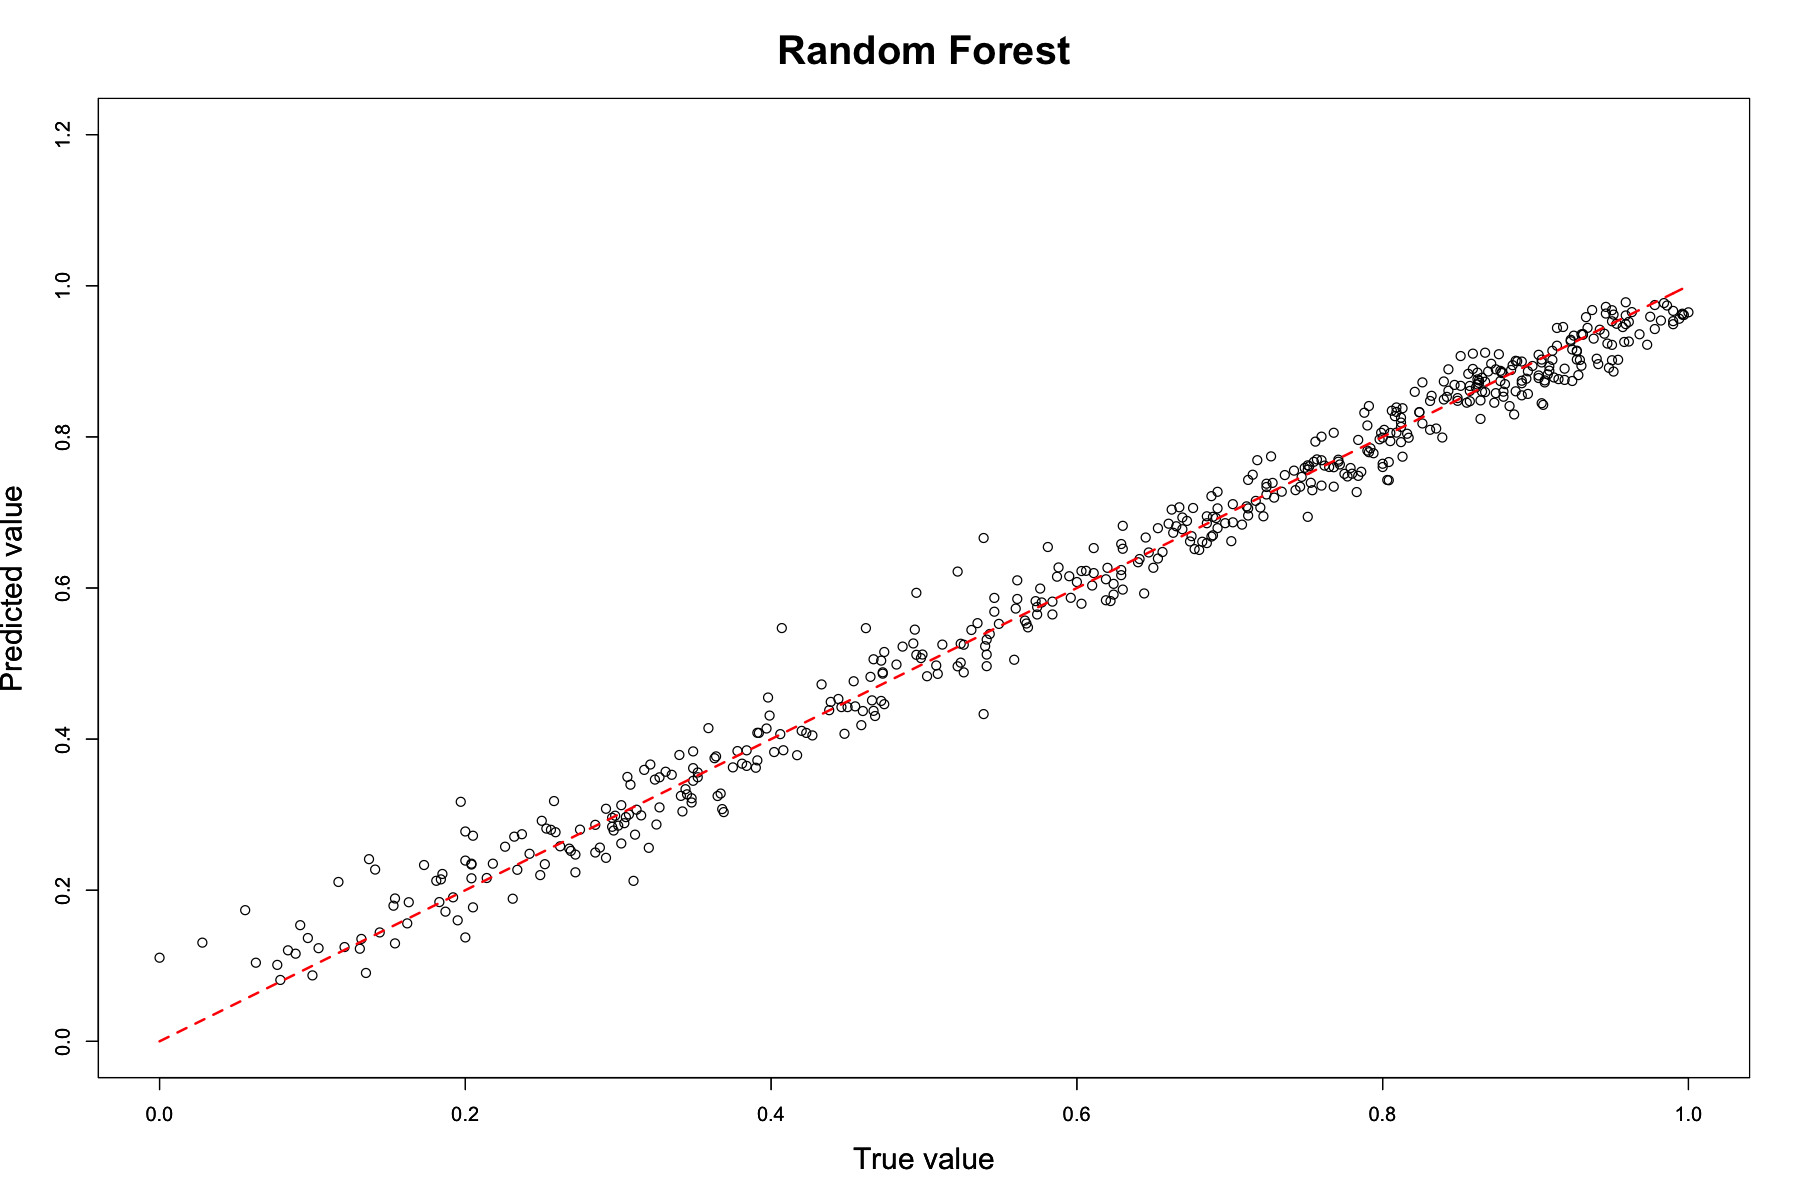
\includegraphics[width = 1.0\textwidth]{Figure/4.2.4-RF.png}
\caption{The predicted Arctic sea ice extent value vs the real Arctic sea ice extent value with Random Forest (200 trees, 5 features). The red referenced dotted line represents the straight line y=x. Mean Square Error (MSE) is 0.00105.}
\label{4.2.4-RF}
\end{figure}



\subsection{Neural Network} %4.2.5

For neural networks, unlike random forests, parameters can be selected based on out-of-pocket errors. Therefore, in the parameter tuning process k-fold is applied to output testing errors for reference. After multiple tests, we finally selected the structure of 5 hidden layers, and 9, 7, 5, 3 and 1 neurons were used in each hidden layer from front to back as following figure shows.

\begin{figure}[htbp]
\centering
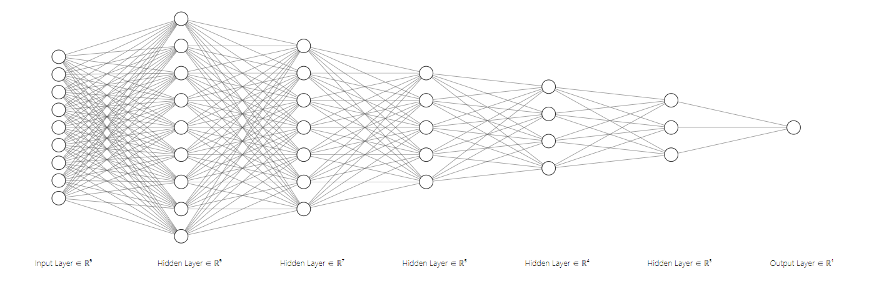
\includegraphics[width = 1.0\textwidth]{Figure/4.2.5-NN-Structure.png}
\caption{Neural Networks Structure}
\label{4.2.5-NN-Structure}
\end{figure}

As for the result, the neural network algorithm achieves excellent performance similar to that of random forest. MSE was slightly lower than the random forest, reaching 1.00104. The fitting diagram (Figure \ref{4.2.5-NN}) also proves that the variance of the neural network model is very low comparing with former algorithms except Random Forest.

\begin{figure}[htbp]
\centering
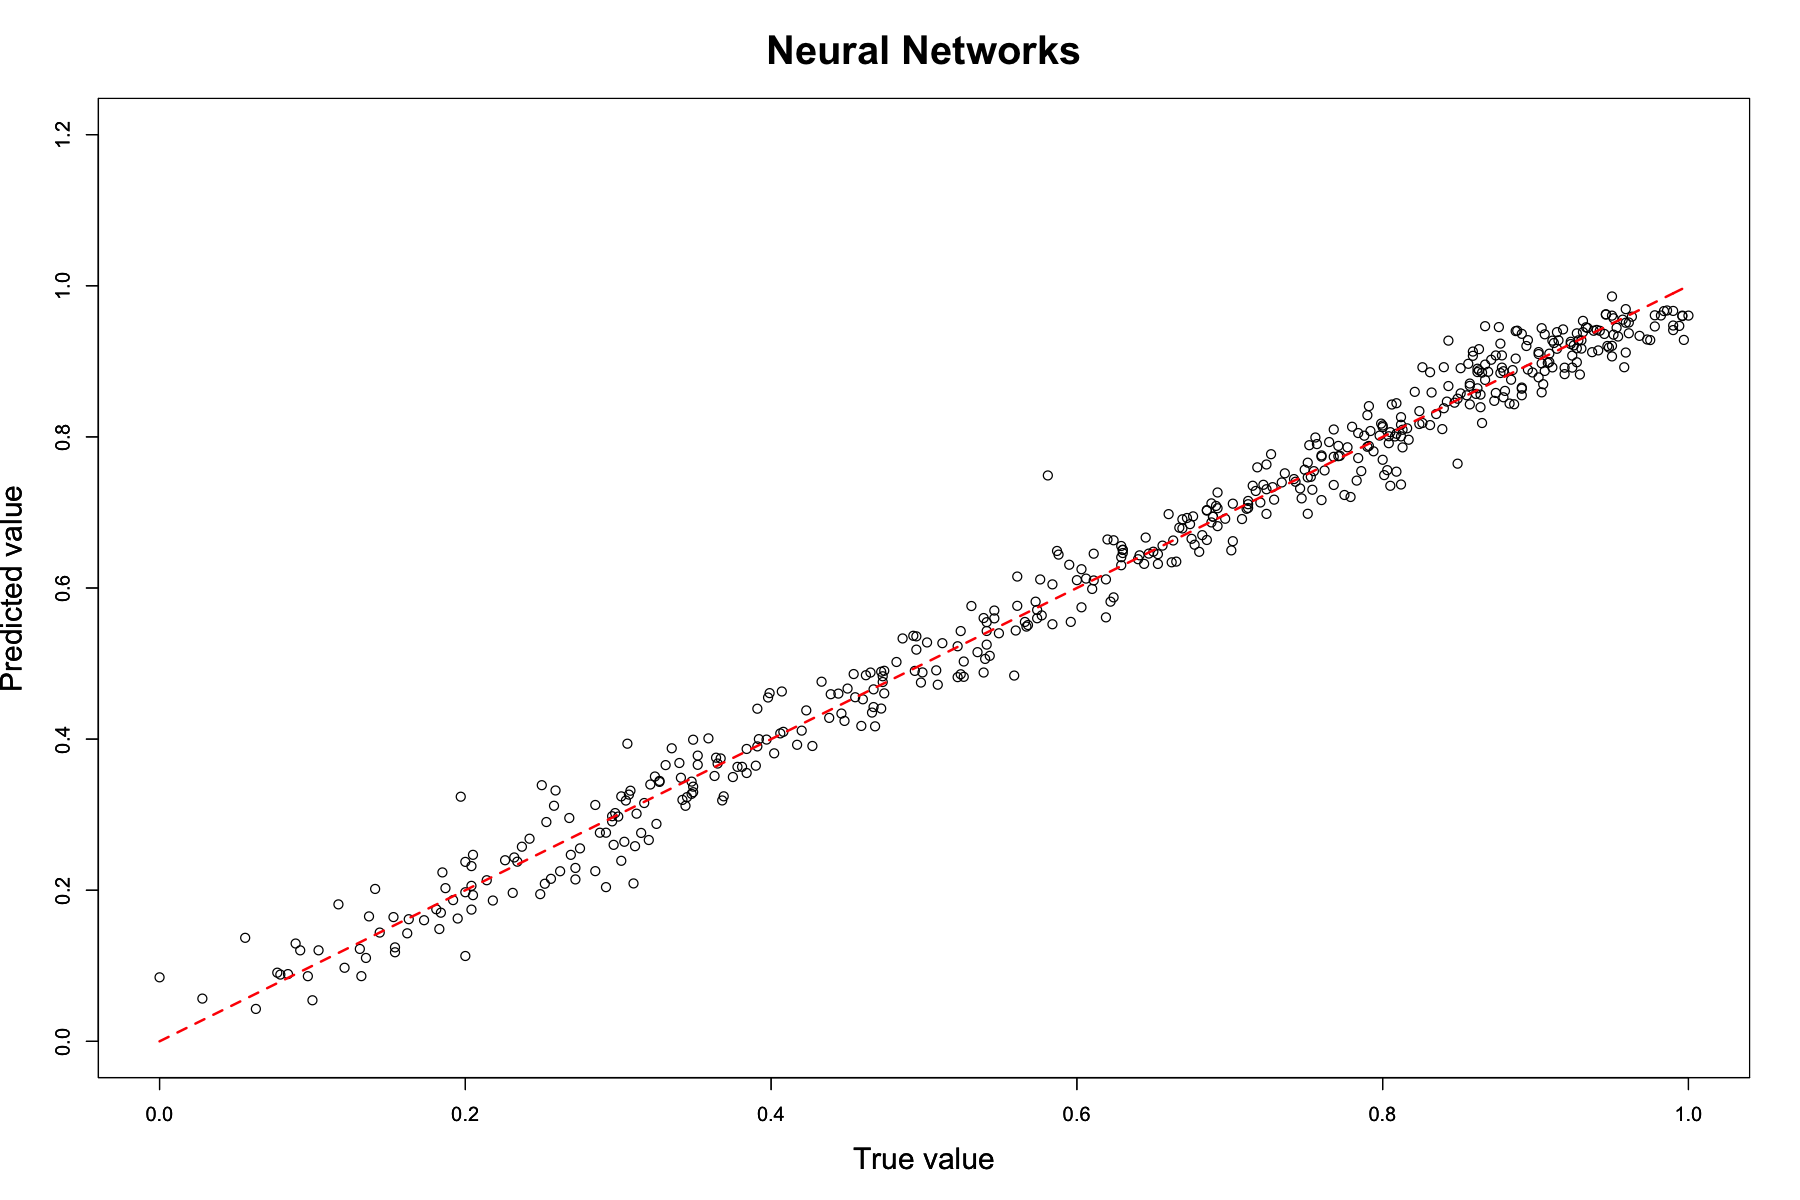
\includegraphics[width = 1.0\textwidth]{Figure/4.2.5-NN.png}
\caption{The predicted Arctic sea ice extent value vs the real Arctic sea ice extent value with Neural Networks (9 neurons, 5 hidden layers with (9,7,5,4,3) nodes respectively). The red referenced dotted line represents the straight line y=x. Mean Square Error (MSE) is 0.00104.}
\label{4.2.5-NN}
\end{figure}



\subsection{Comparison} %4.2.6
Based on the above four models and seven prediction results, all the results are listed and compared here. 

**TABLE**
\begin{figure}[htbp]
\centering
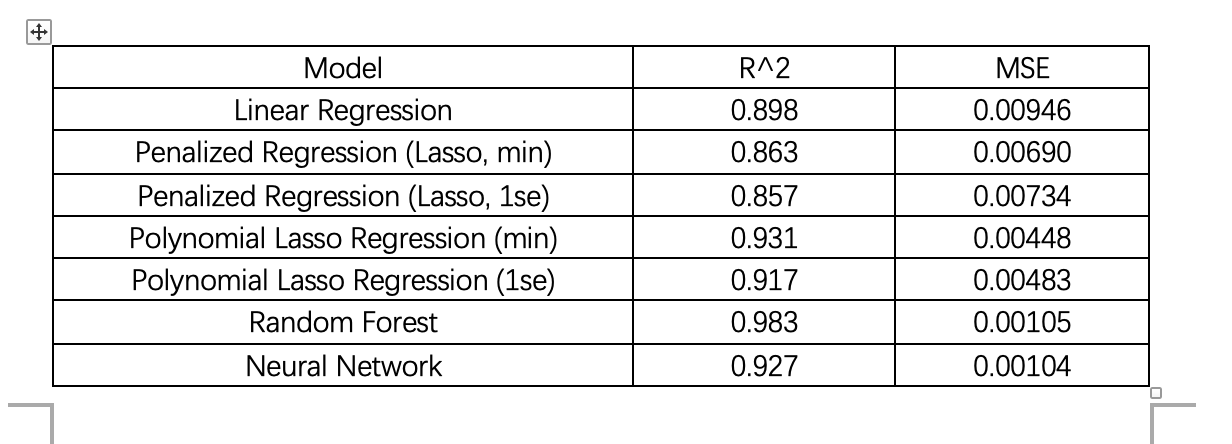
\includegraphics[width = 1.0\textwidth]{Figure/4.2.6-TABLE.png}
\caption{4.2.6-TABLE}
\label{4.2.6-TABLE}
\end{figure}

First, Random Forest, as the best performing model, will be selected for further future predictions. Secondly, it can be found that the model with high $\text{R}^2$ may not perform well, which also proves the existence of over-fitting phenomenon and the necessity of penalise.
\section{Sea Ice Future Forecasting} %4.3

\subsection{Normal Situation} %4.3.1




\subsection{Emergency Situation} %4.3.2


\chapter{Discussion}                            % Chapter 5
\label{Chapter5:Discussion}
% section:
% Chapter 5: Discussion




\chapter{Conclusion}                            % Chapter 5
\label{Chapter6:Conclusion}
% section:
% Chapter 5: Conclusion






% Bibliography
\bibliographystyle{IEEEtran}
\bibliography{ref}

\end{document}